\documentclass[12pt,a4paper]{article}
\usepackage[utf8]{inputenc}
\usepackage{graphicx}
\usepackage{geometry}
\usepackage{fancyhdr}
\usepackage{listings}
\usepackage{xcolor}
\usepackage{float}
\usepackage[colorlinks=false,hidelinks]{hyperref}

\geometry{margin=1in}
\pagestyle{fancy}
\fancyhf{}
\rhead{FIT5032 - Assessed Lab 10}
\cfoot{\thepage}

% Code listing style
\lstset{
    basicstyle=\ttfamily\small,
    breaklines=true,
    frame=single,
    numbers=left,
    numberstyle=\tiny,
    commentstyle=\color{green!50!black},
    keywordstyle=\color{blue},
    stringstyle=\color{red}
}

\title{FIT5032 Assessed Lab 10\\
External API Services \& Local API Development}
\author{Student Name: [Du Daoan]\\
Student ID: [35523166]}
\date{}

\begin{document}

\maketitle

\tableofcontents
\newpage

\section{EFOLIO TASK 10.1 (PASS AND CREDIT LEVEL)}

\subsection{Screenshot Set 1: Current Location Weather}

\subsubsection{Weather Application Code Implementation}
% Screenshot showing WeatherView.vue code with API integration
%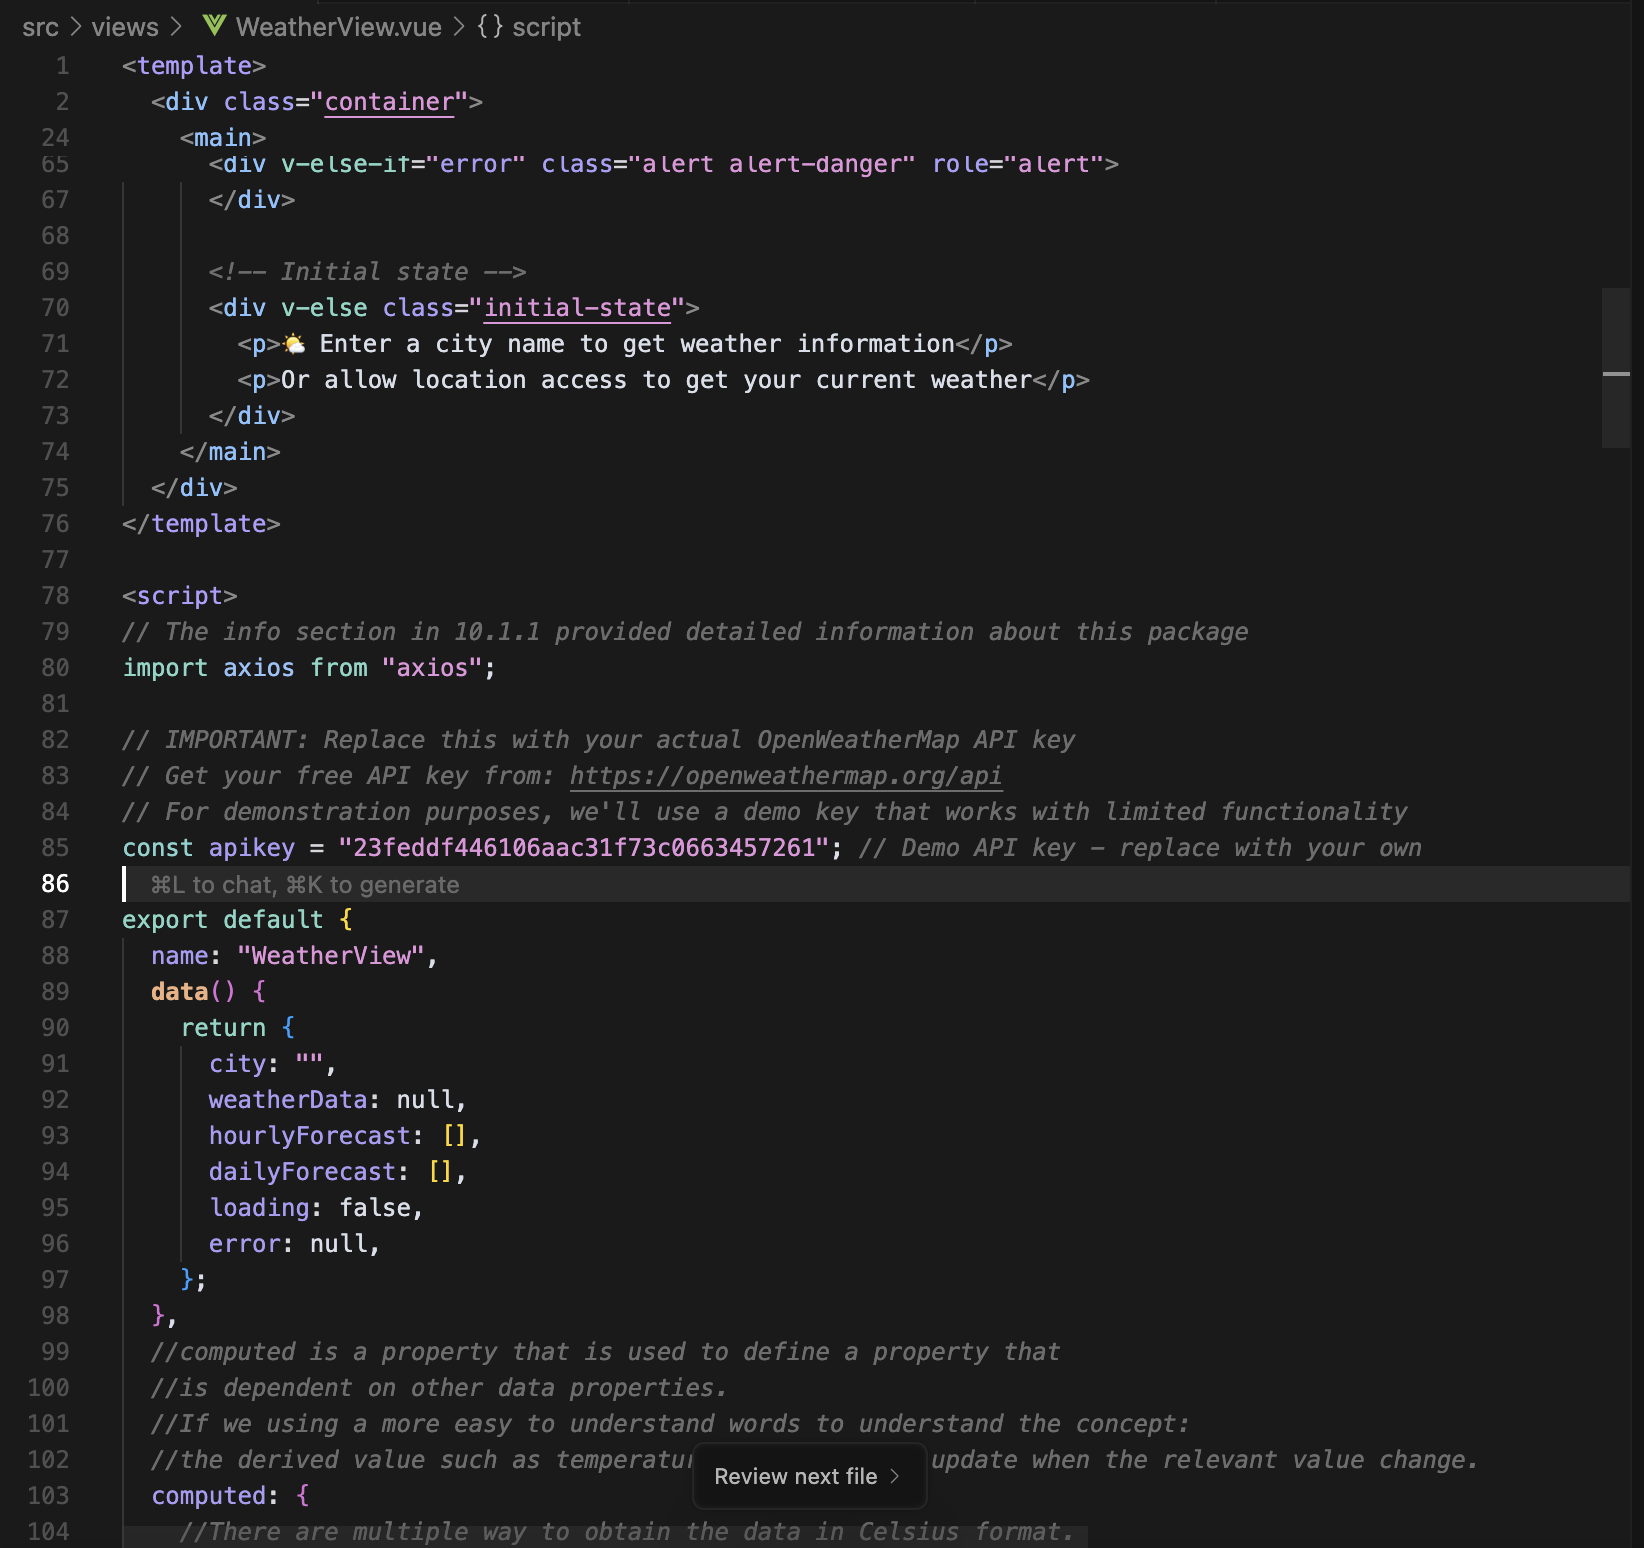
\includegraphics[width=0.9\textwidth]{weather_code_implementation.png}
\begin{figure}[H]
\centering
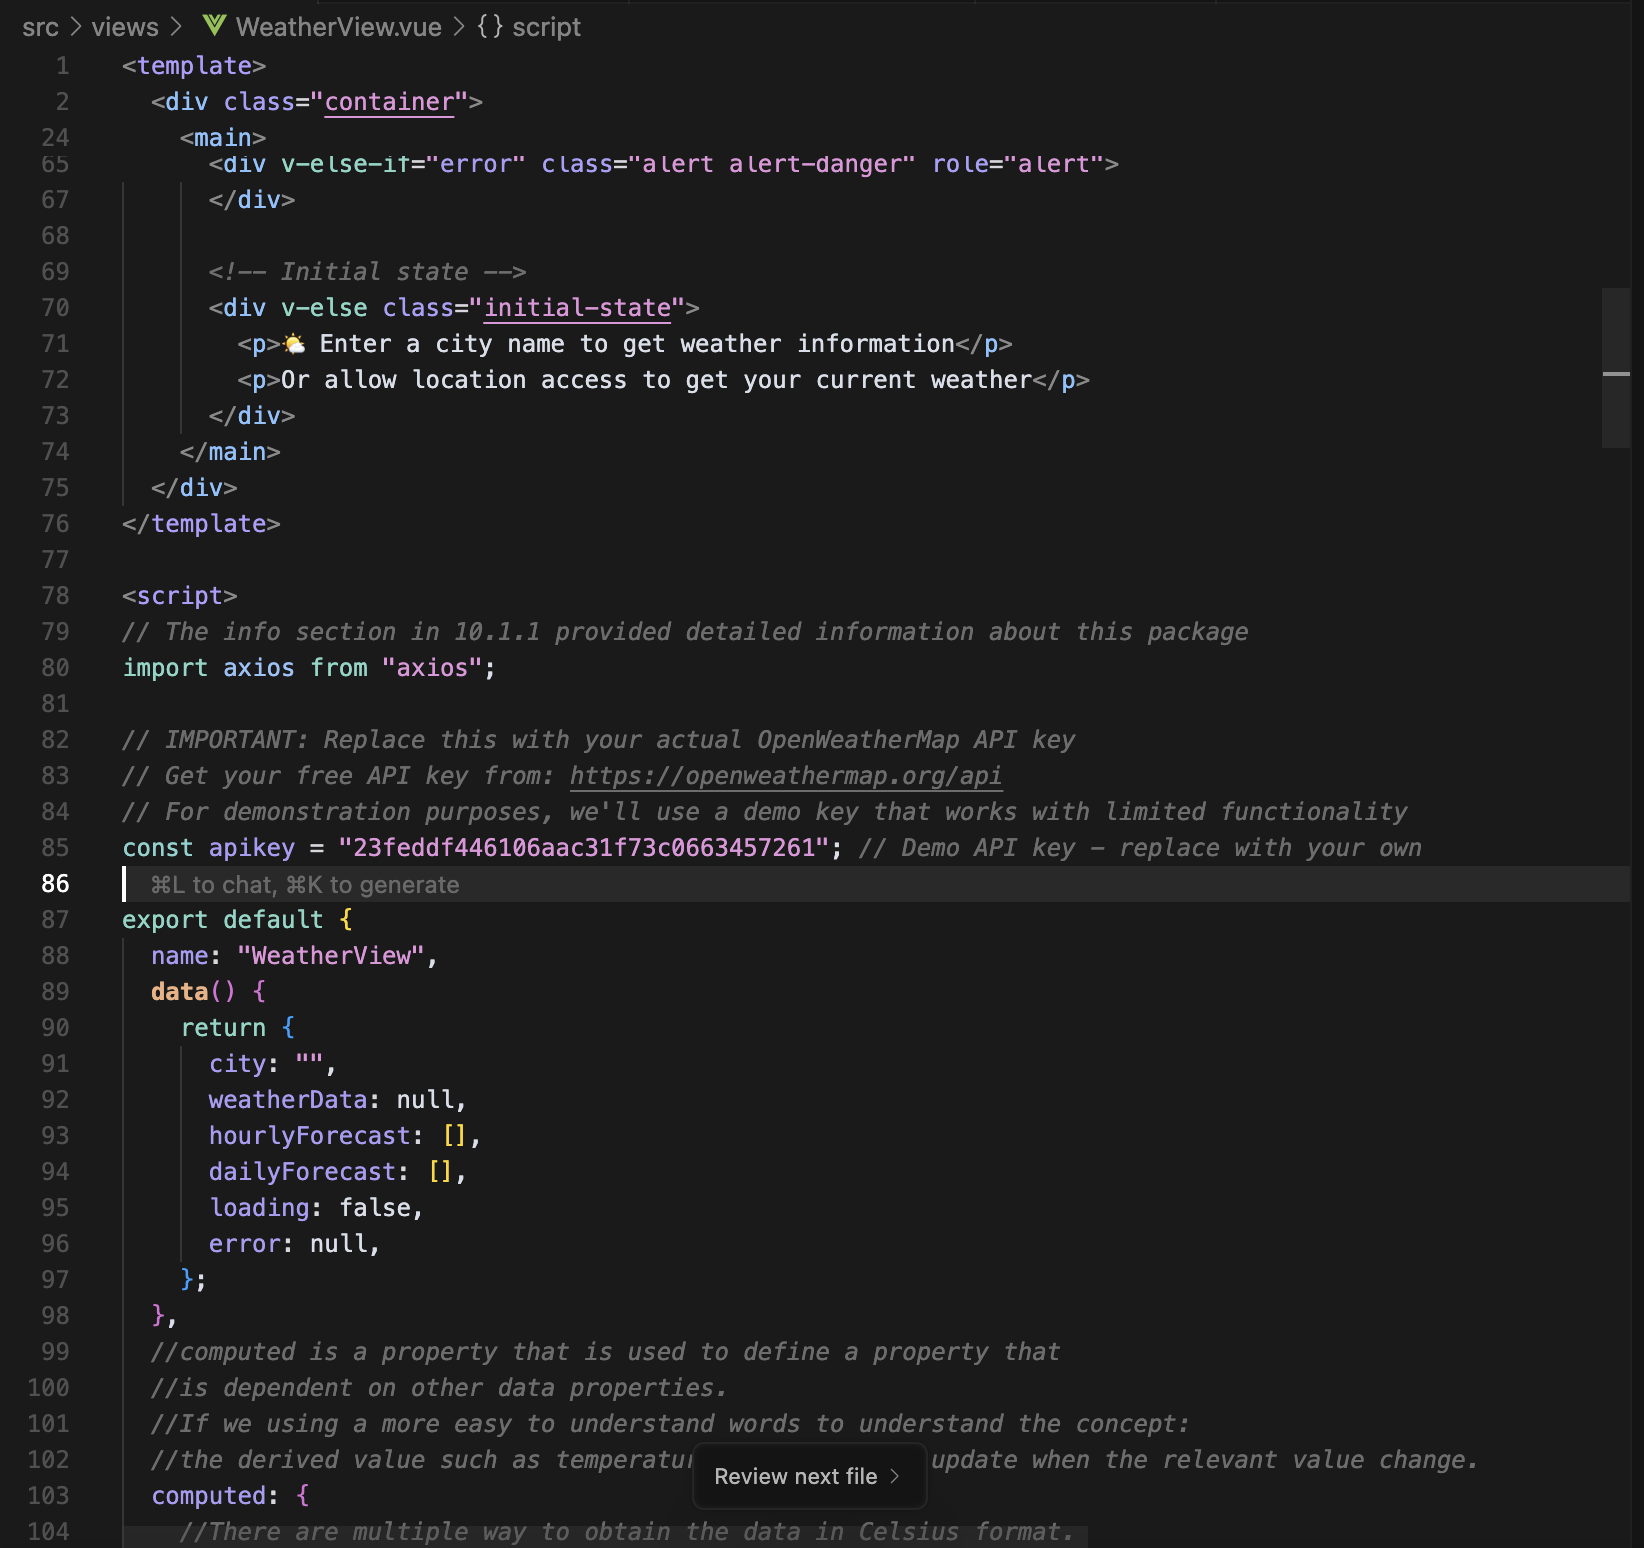
\includegraphics[width=0.9\textwidth]{weather_code_implementation.png}
\caption{WeatherView.vue - Weather API implementation code showing axios integration and geolocation}
\end{figure}

\subsubsection{Browser Display - Current Location Weather}
% Screenshot showing browser with current location weather data
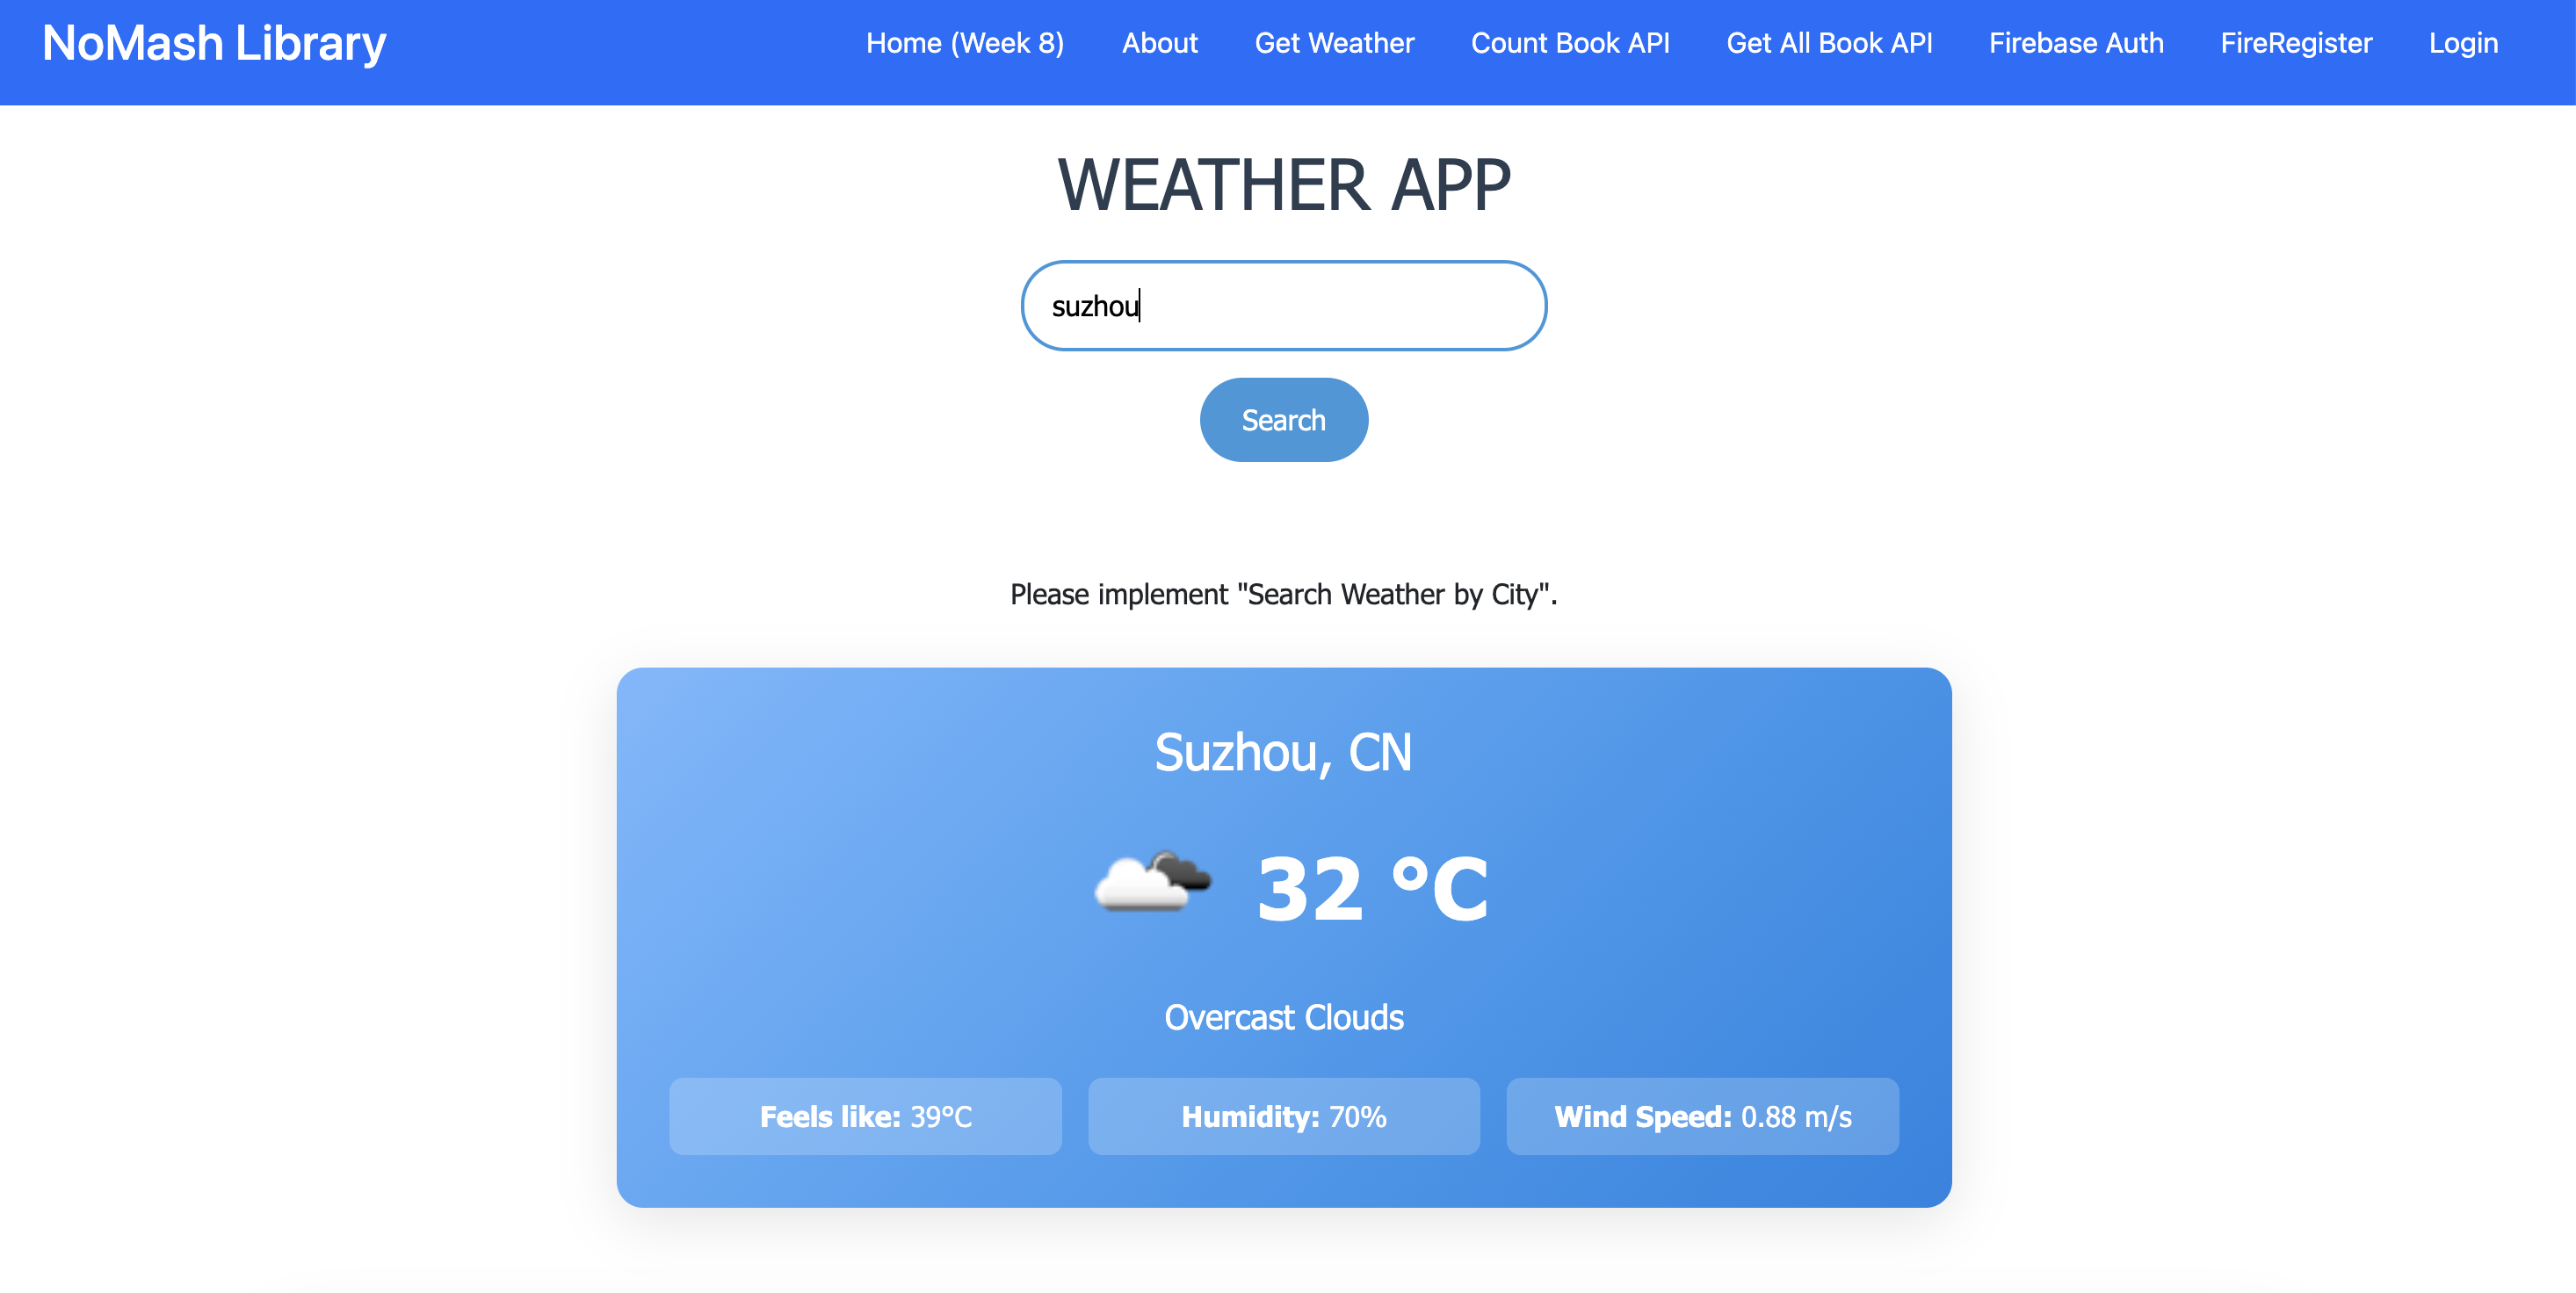
\includegraphics[width=0.9\textwidth]{current_location_weather_browser.png}
\begin{figure}[H]
\centering
% 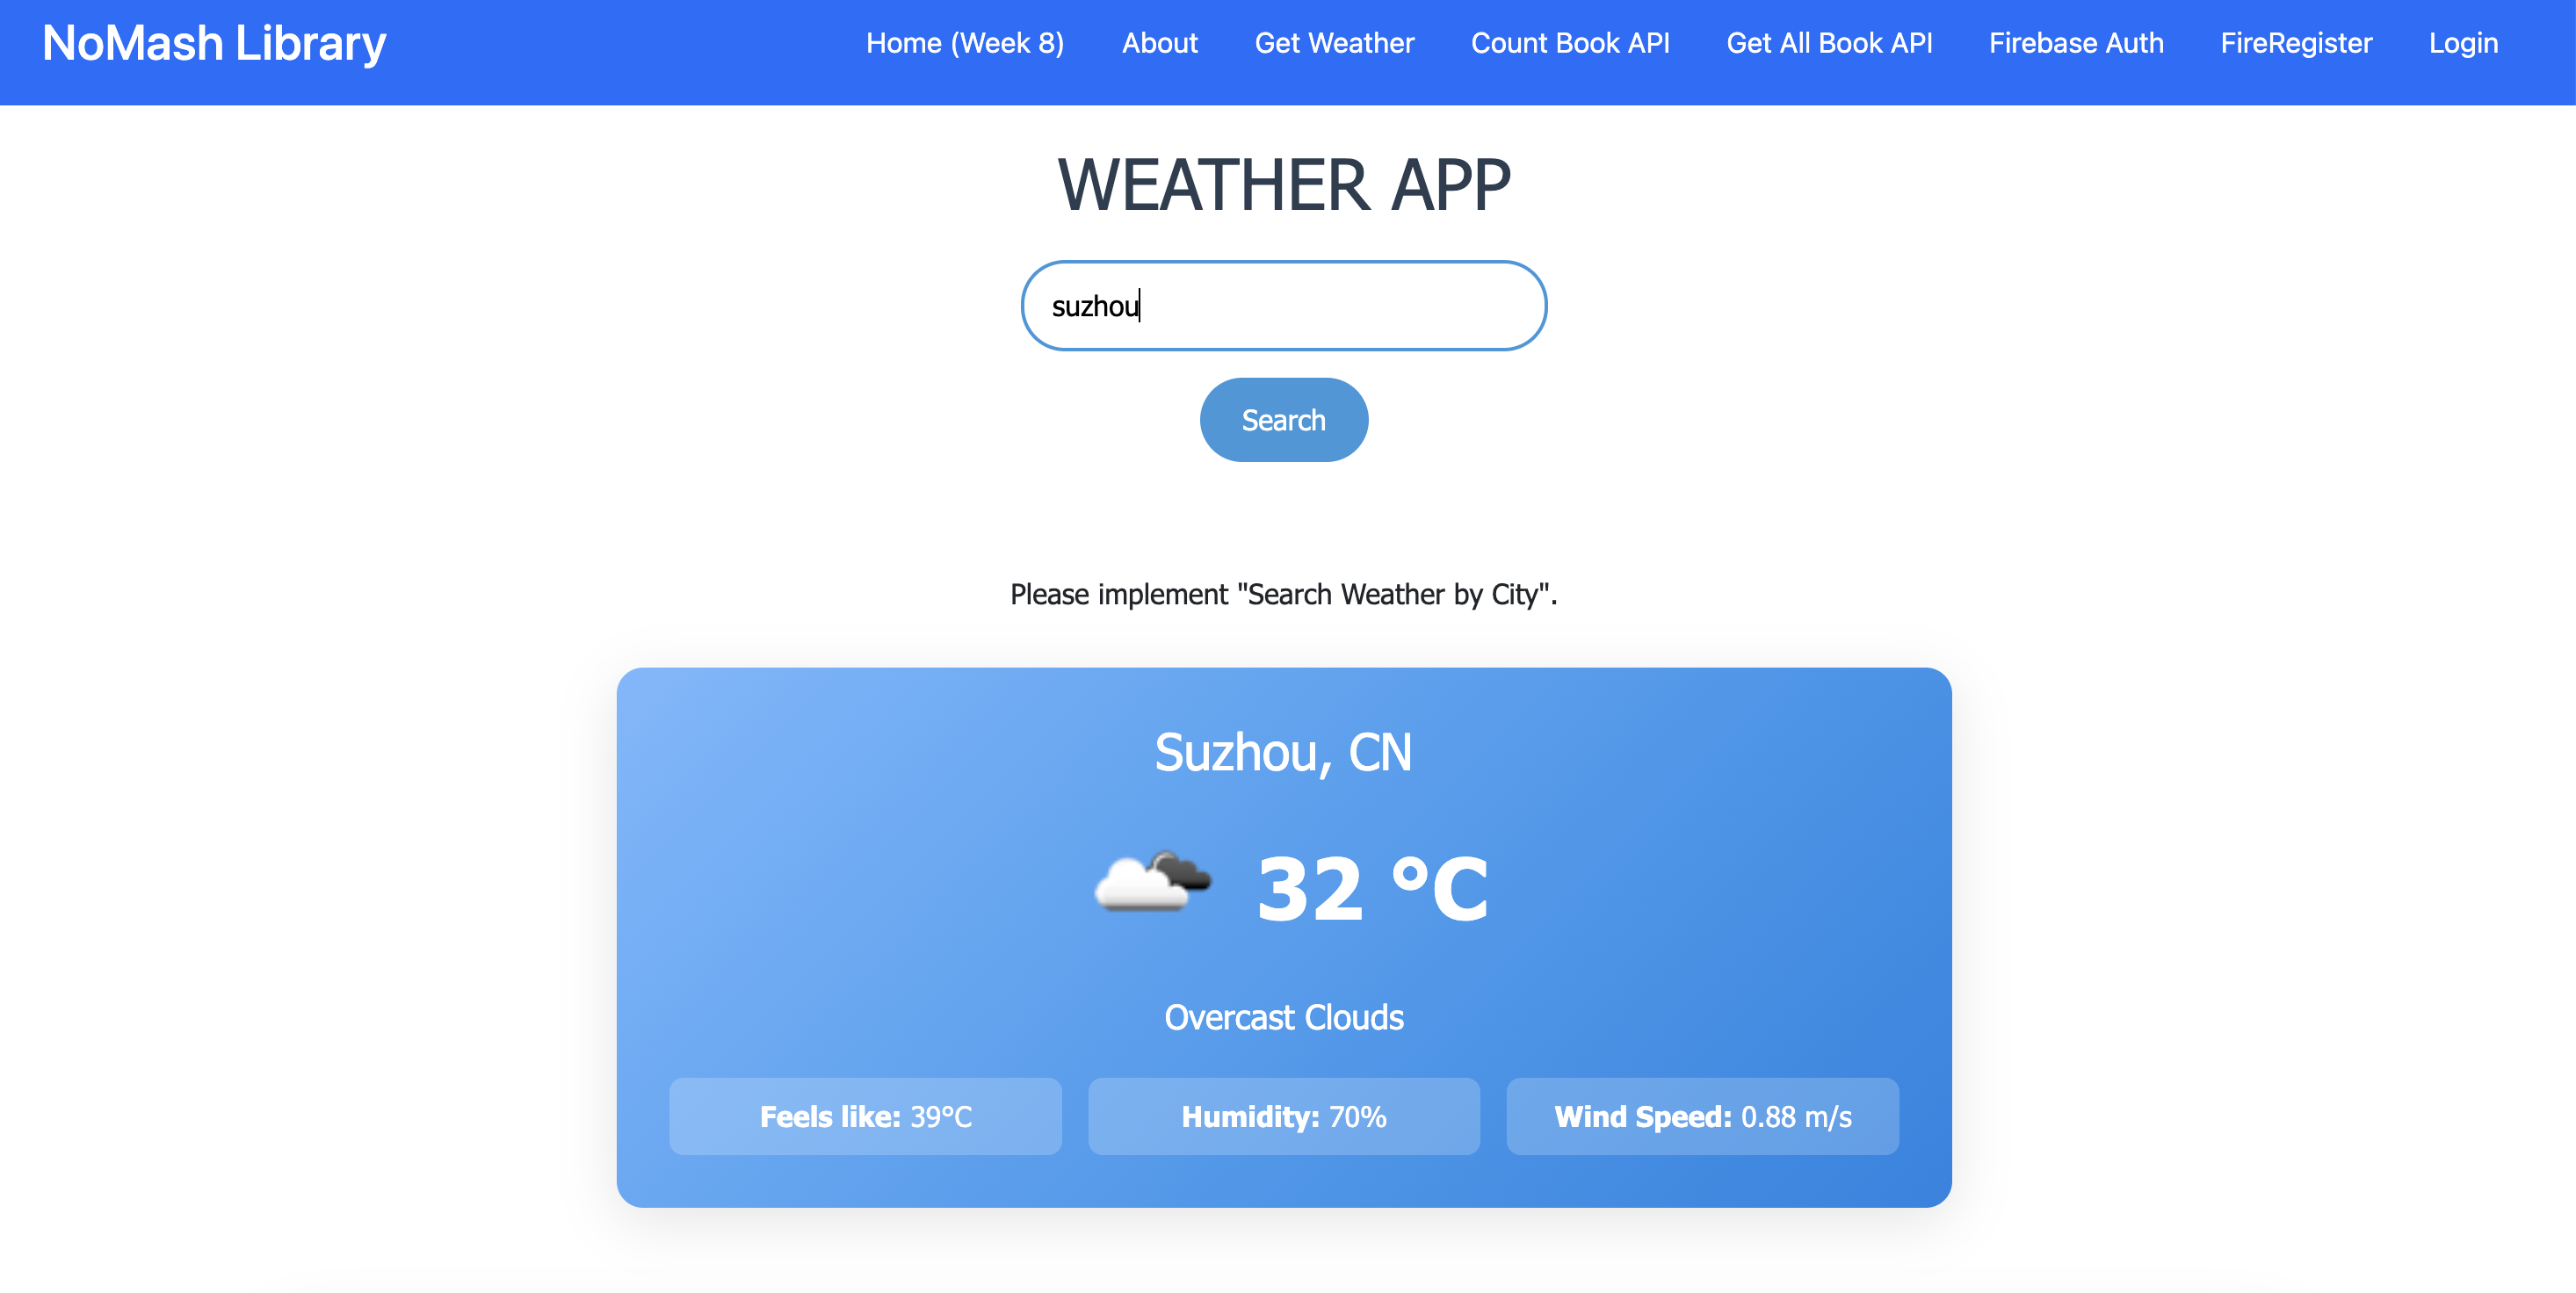
\includegraphics[width=0.9\textwidth]{current_location_weather_browser.png}
\caption{Browser view showing current location weather with temperature in Celsius and weather icon}
\end{figure}

\subsection{Screenshot Set 2: API Page - Authors and Books Count}

\subsubsection{CountBookAPI Code Implementation}
% Screenshot showing CountBookAPI.vue code
% 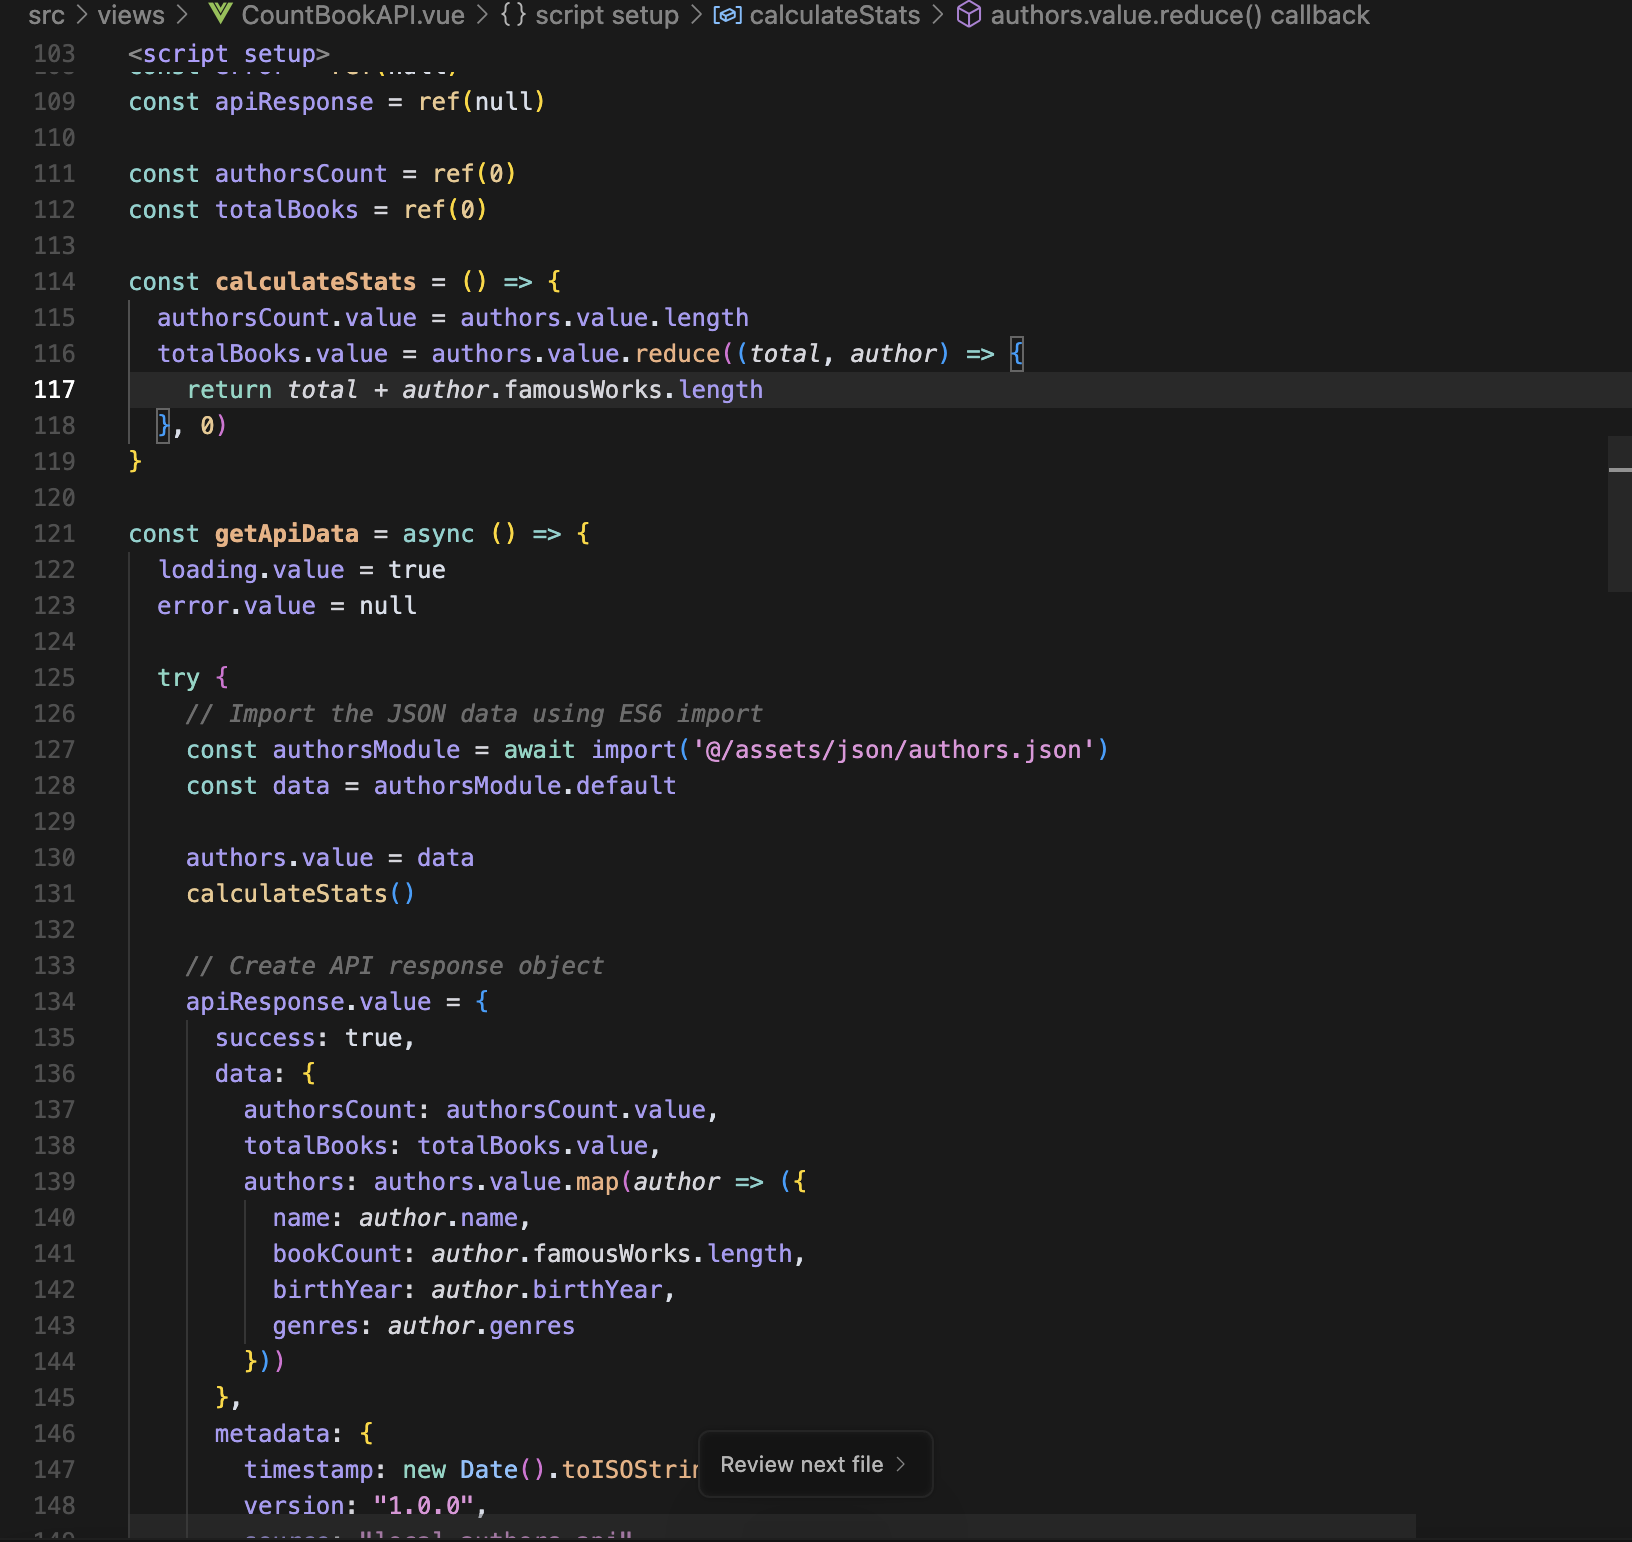
\includegraphics[width=0.9\textwidth]{countbook_api_code.png}
\begin{figure}[H]
\centering
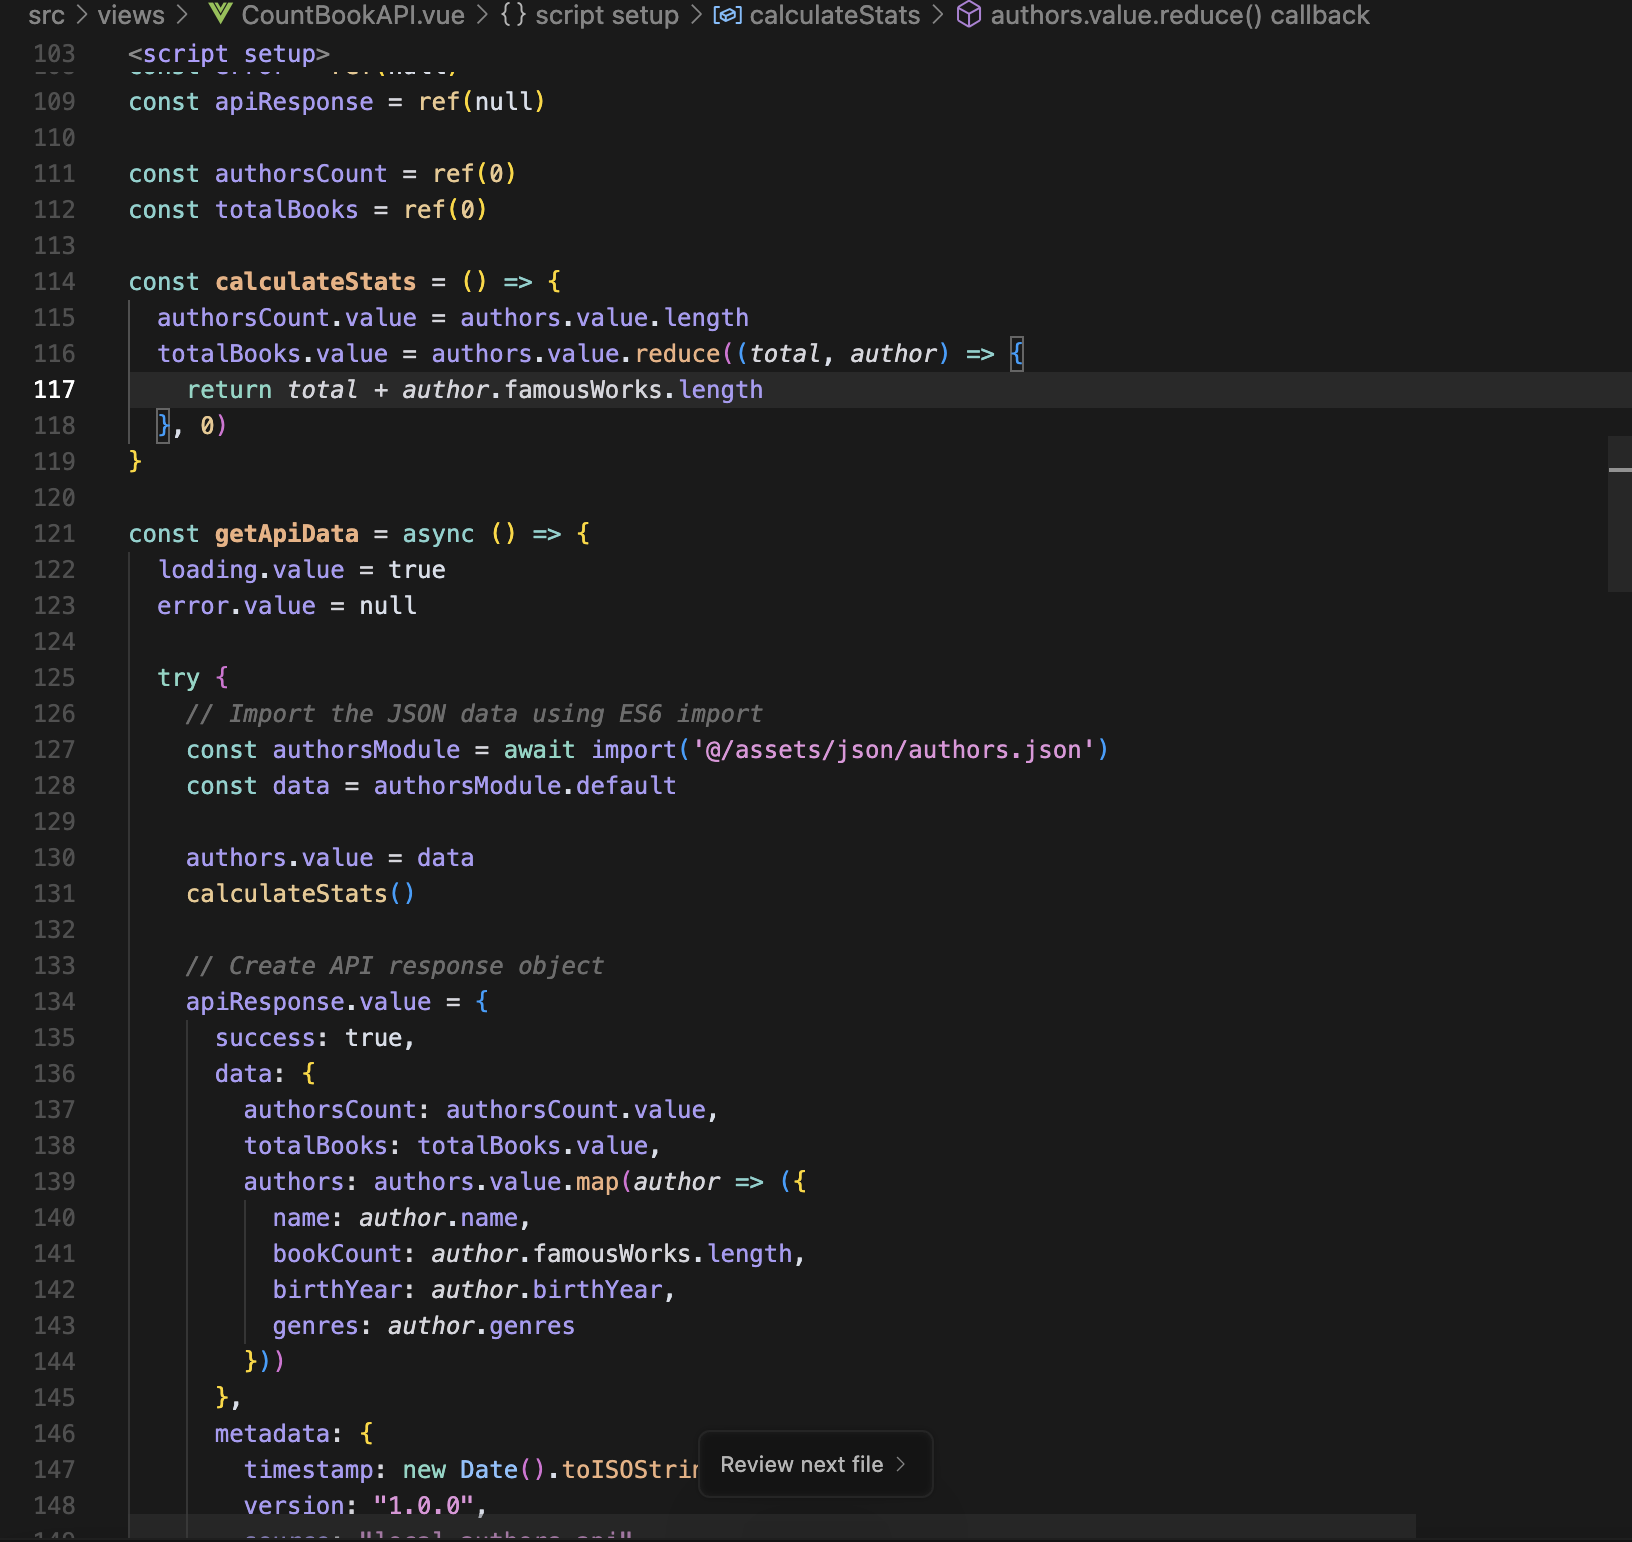
\includegraphics[width=0.9\textwidth]{countbook_api_code.png}
\caption{CountBookAPI.vue - Local API implementation showing JSON data processing}
\end{figure}

\subsubsection{Browser Display - Authors and Books Statistics}
% Screenshot showing browser with authors and books count
% 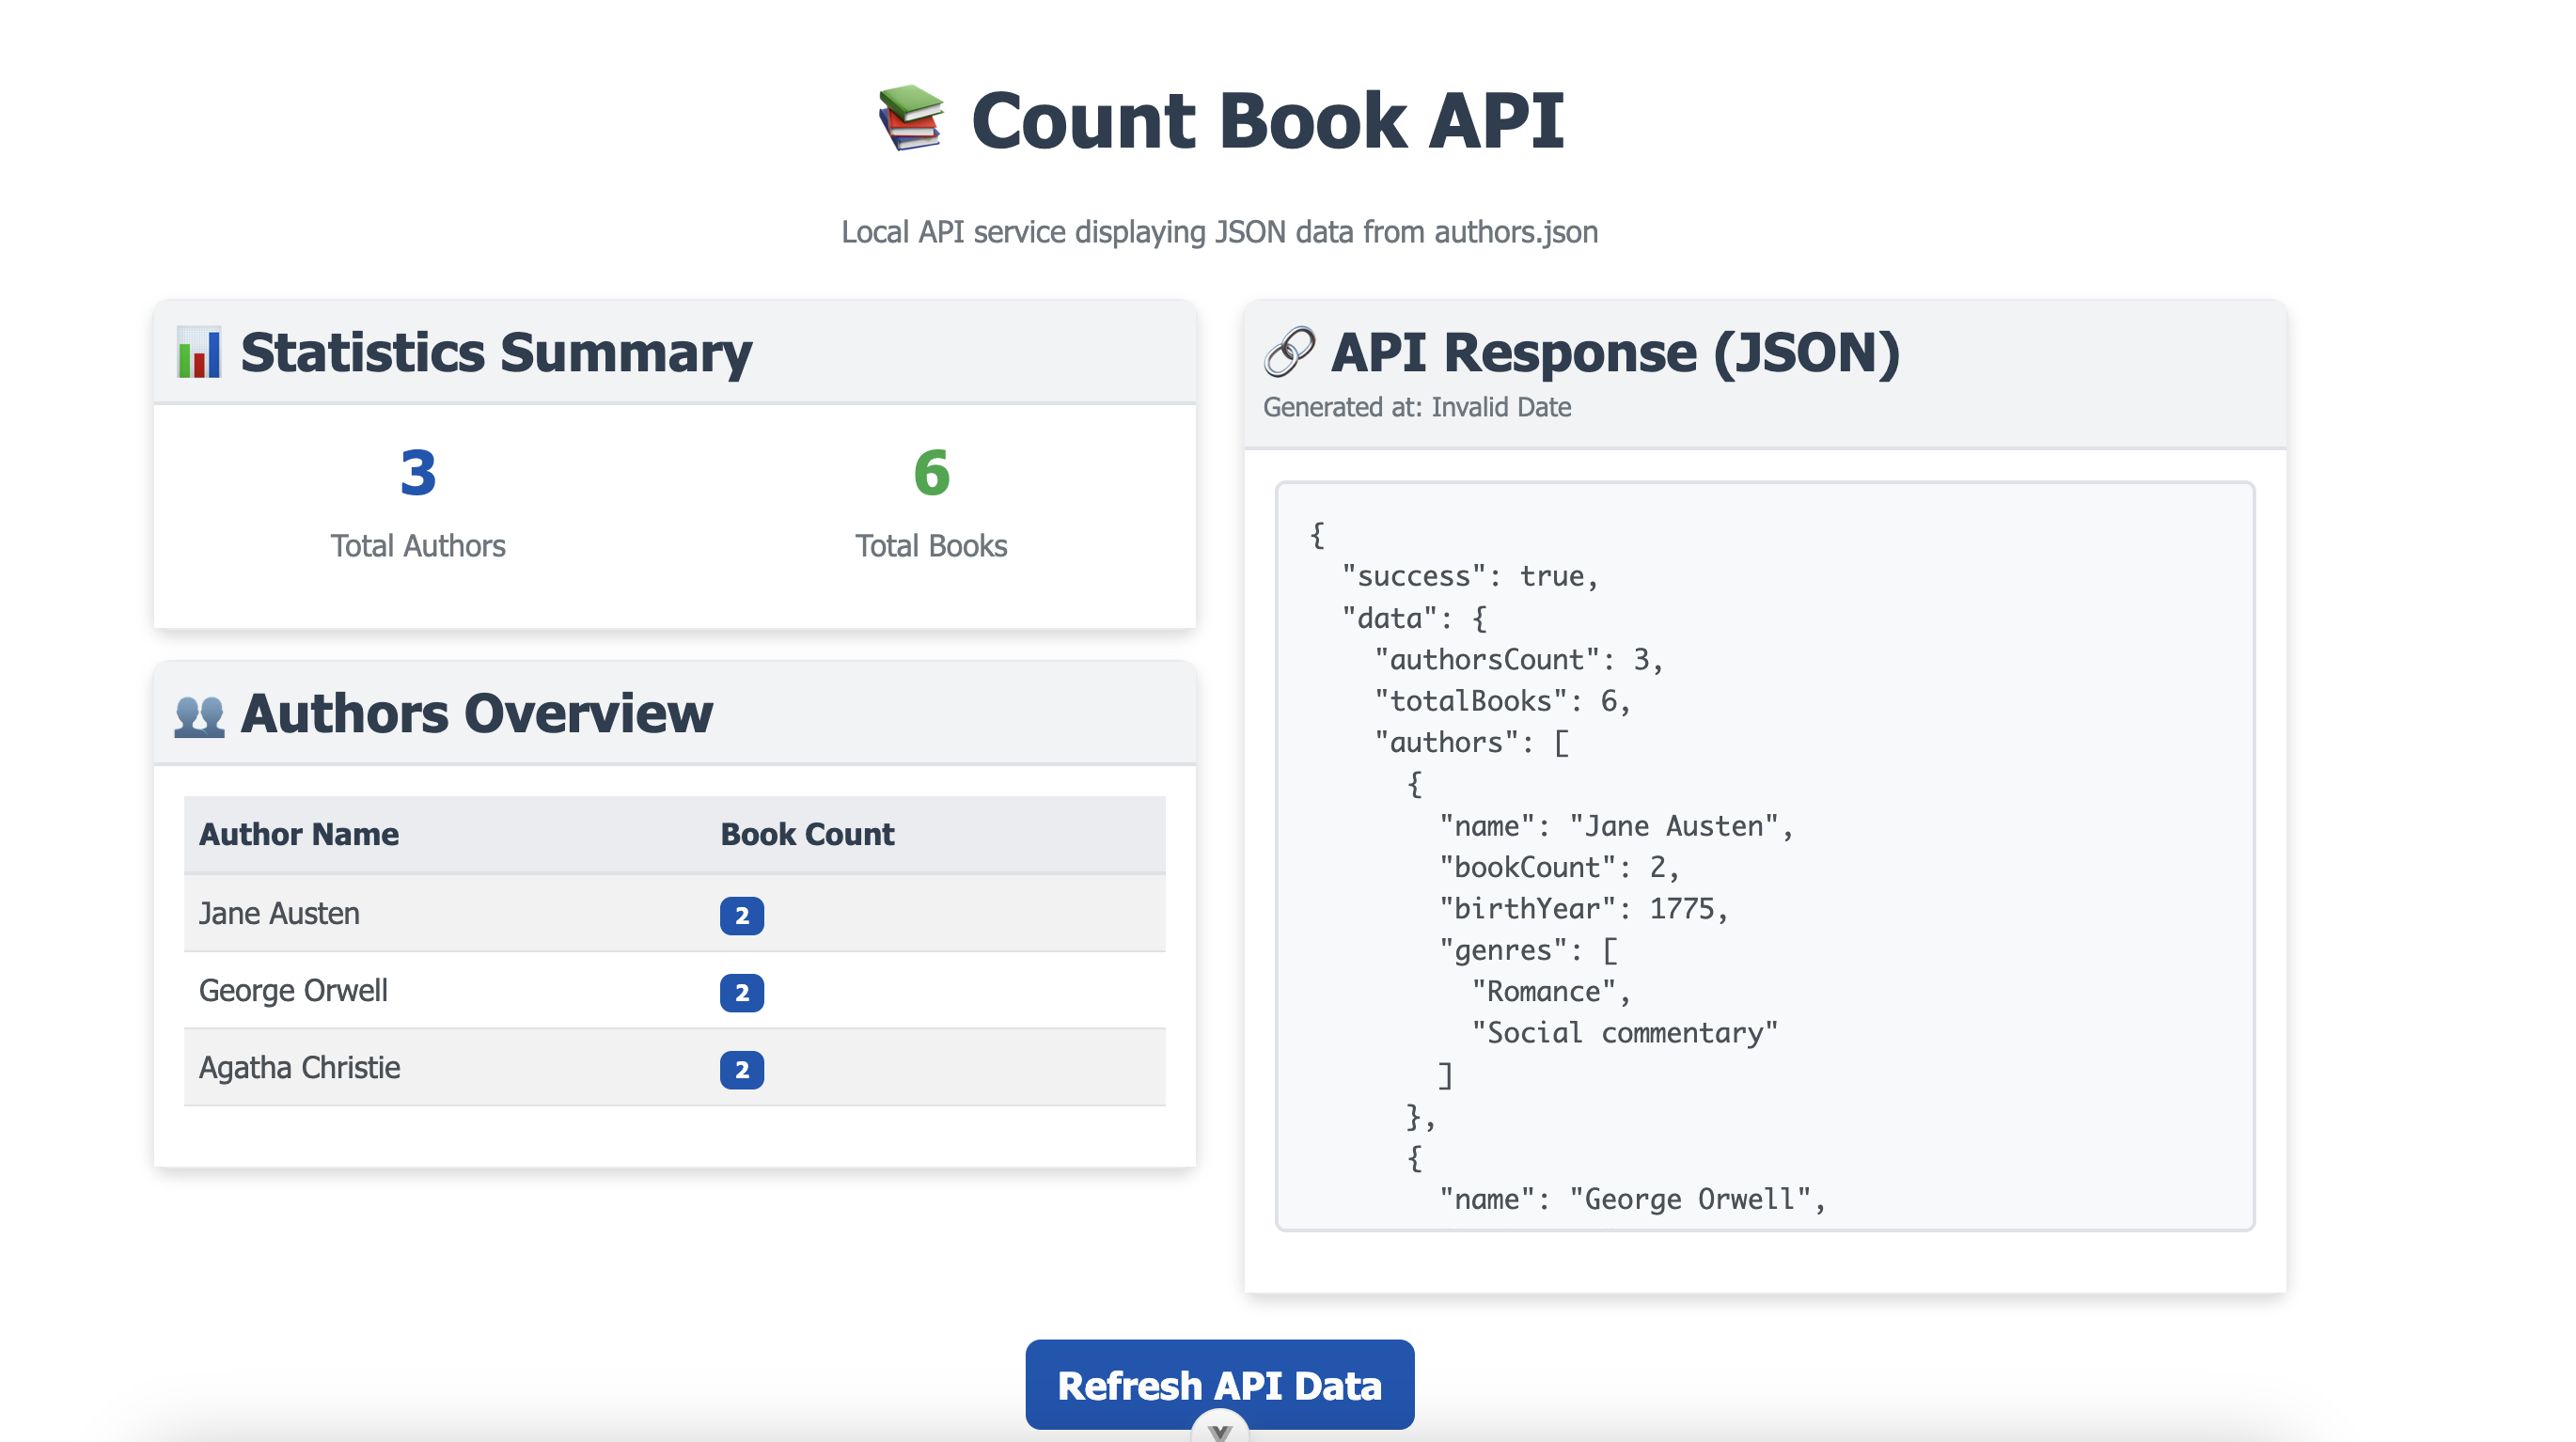
\includegraphics[width=0.9\textwidth]{authors_books_count_browser.png}
\begin{figure}[H]
\centering
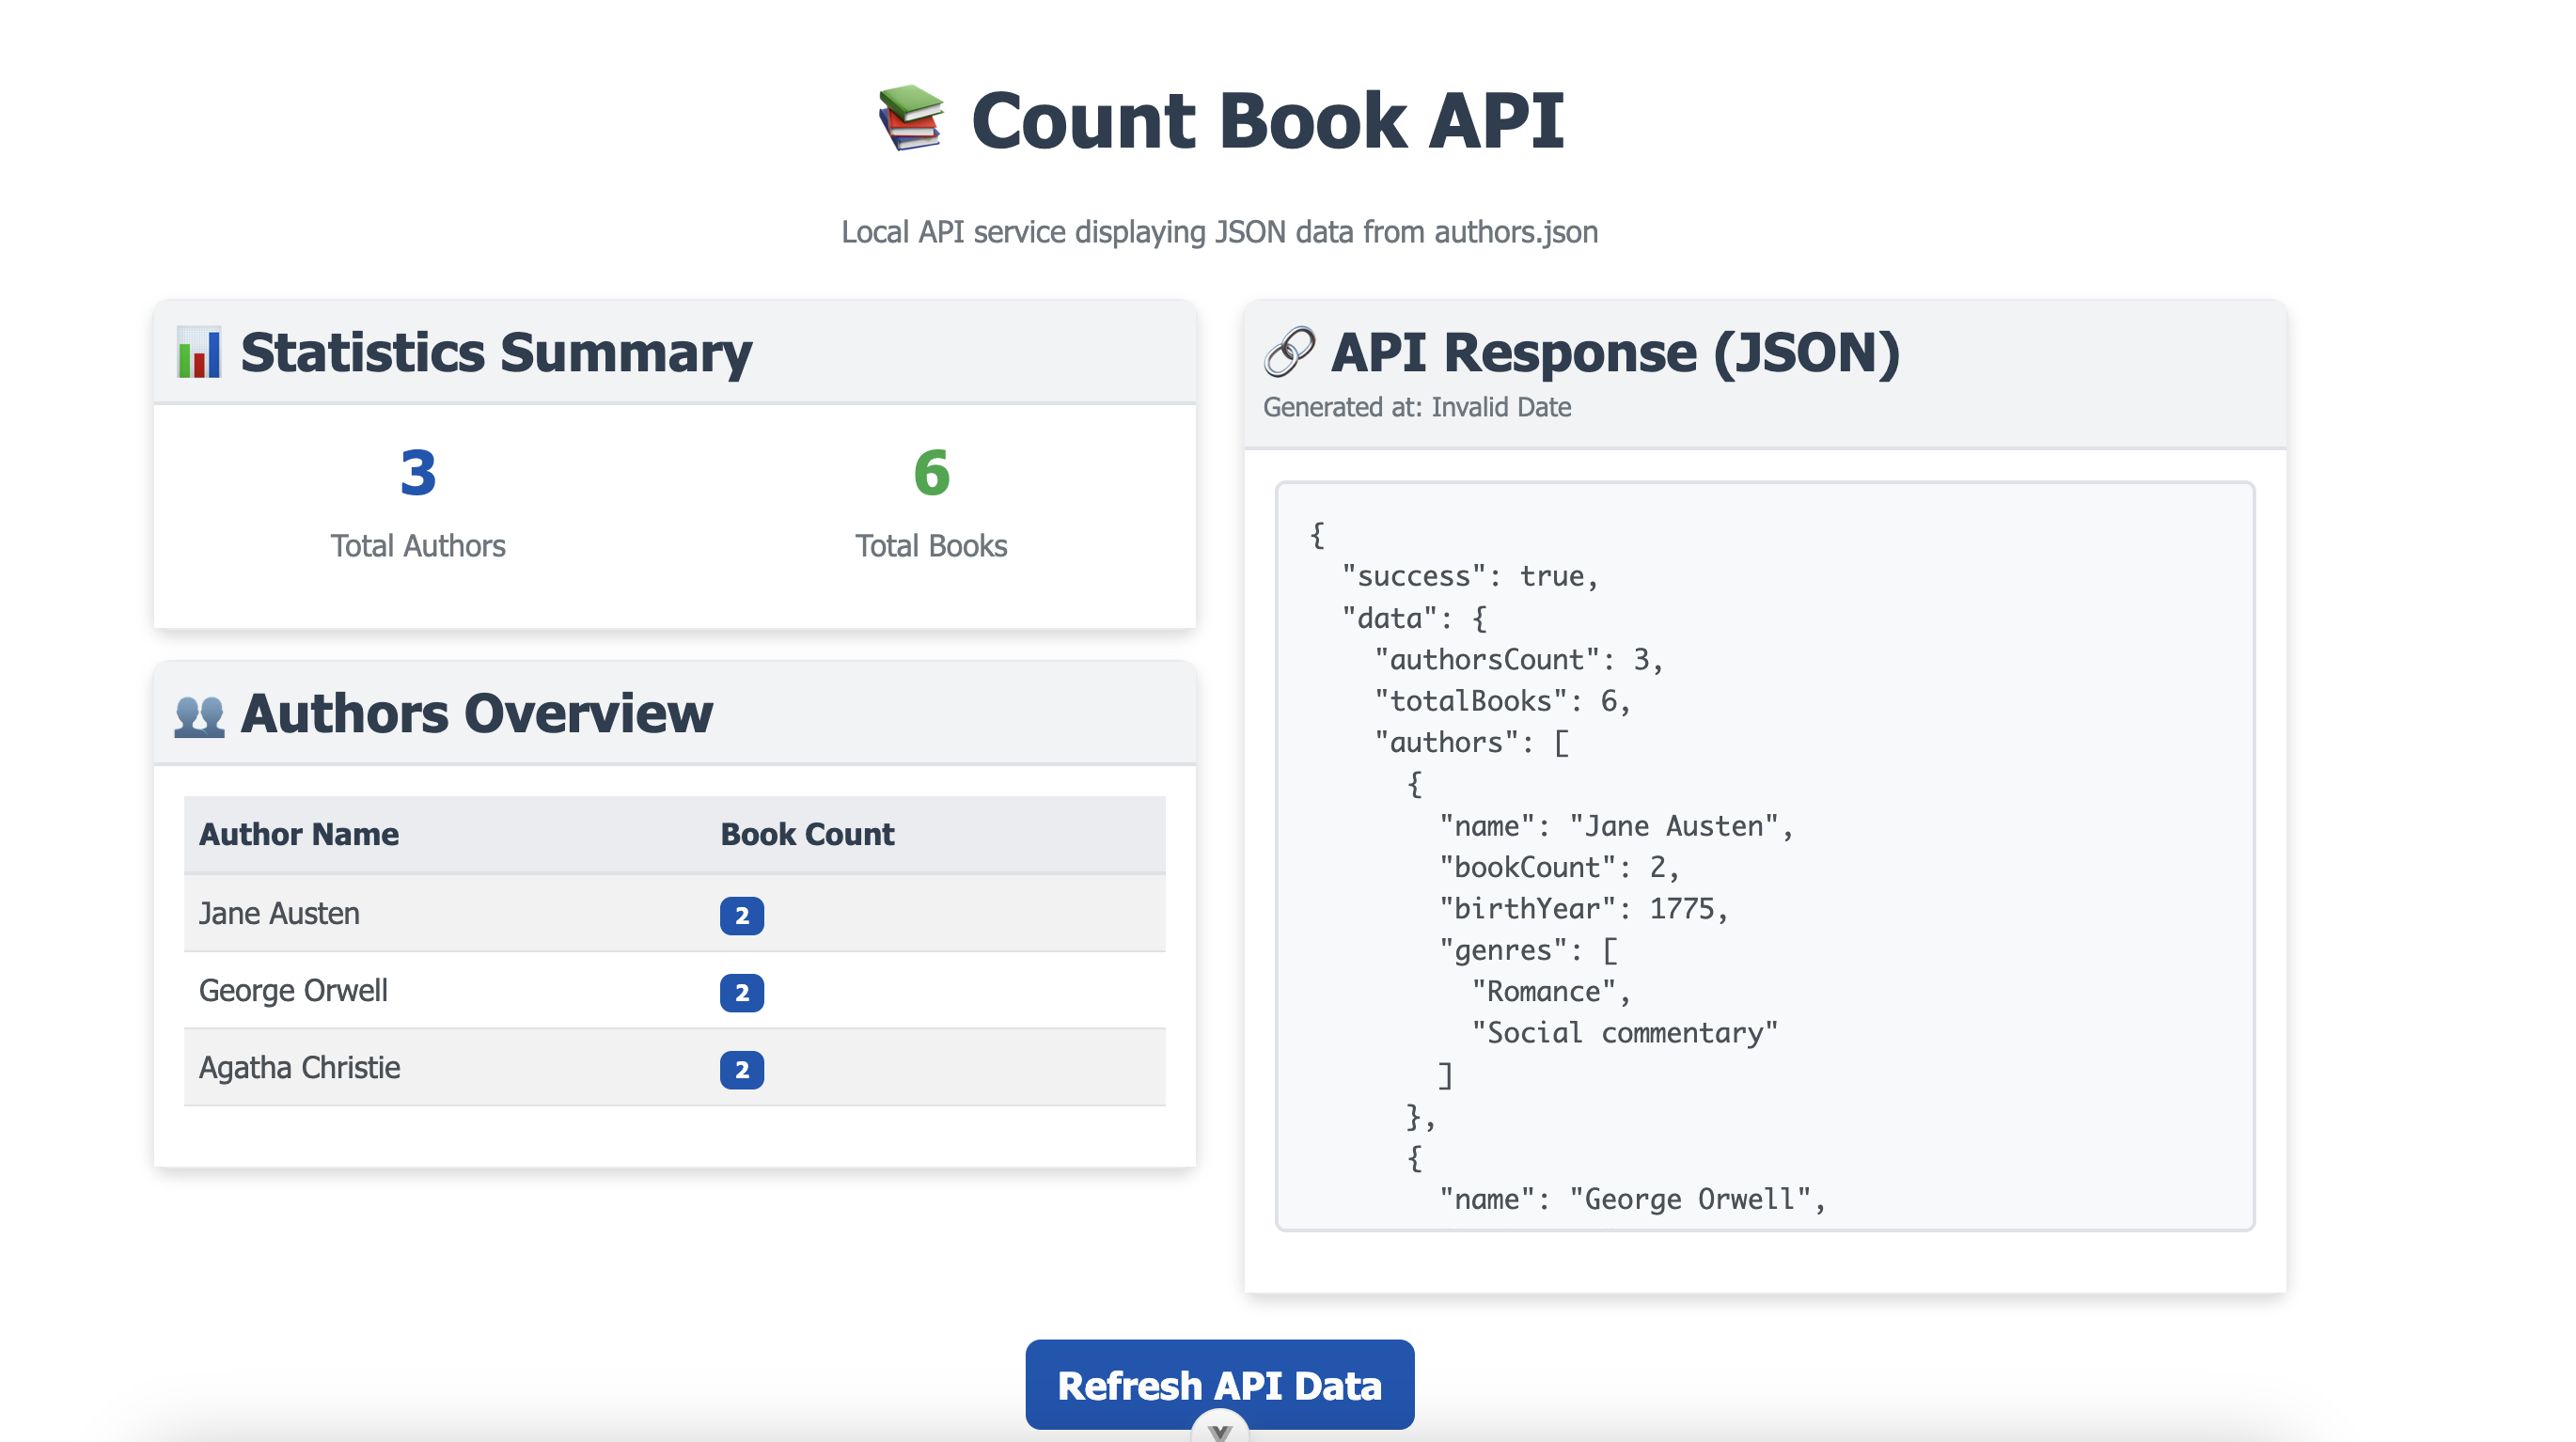
\includegraphics[width=0.9\textwidth]{authors_books_count_browser.png}
\caption{Browser view showing number of authors (3) and total books (6) from authors.json}
\end{figure}

\newpage

\section{EFOLIO TASK 10.2 (DISTINCTION AND HIGH DISTINCTION LEVEL)}

\subsection{Screenshot Set 1: Weather Search by City}

\subsubsection{Weather Search Code Implementation}
% Screenshot showing searchByCity function code
% 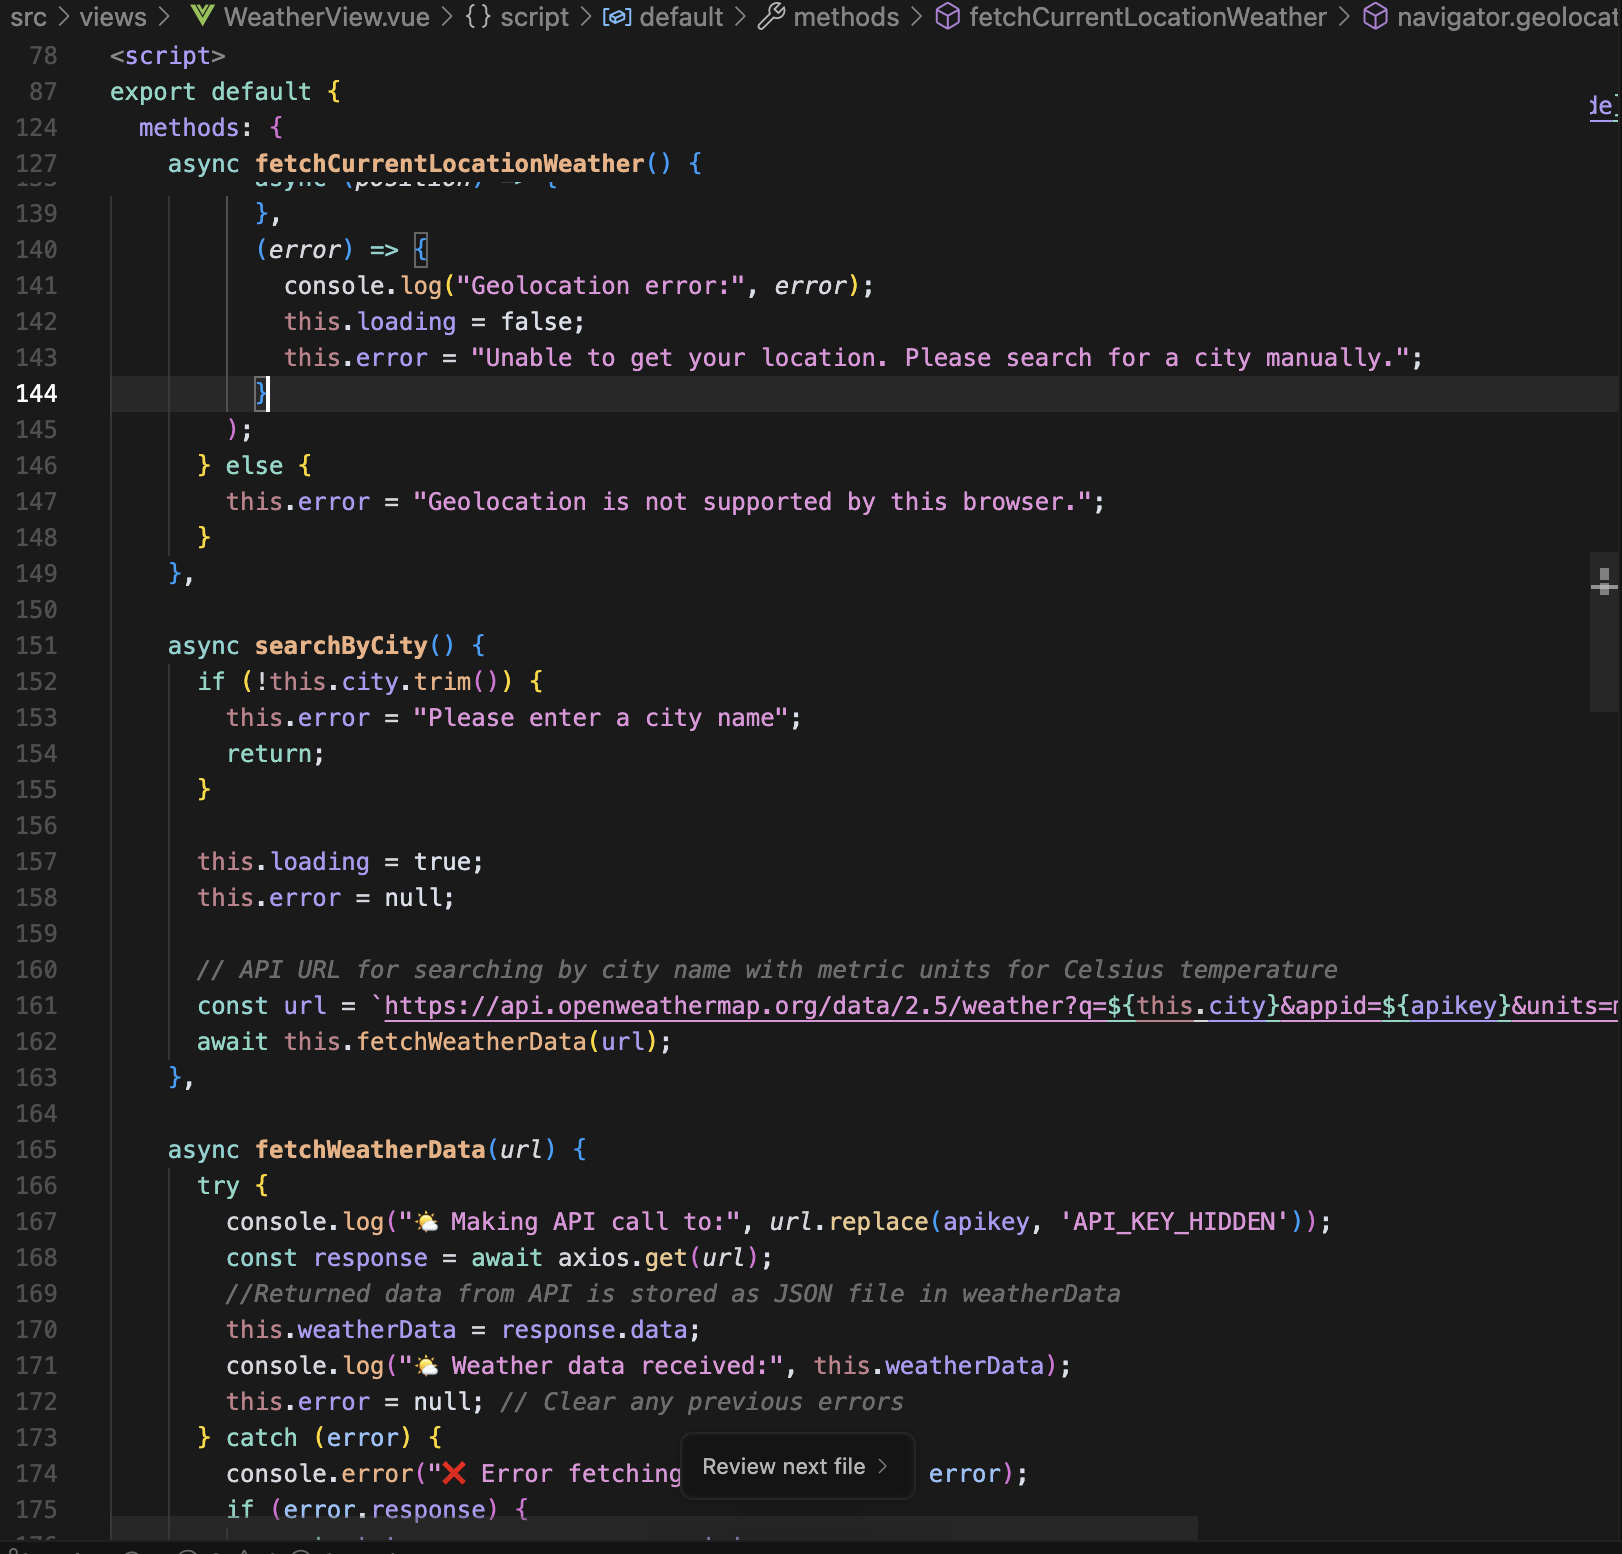
\includegraphics[width=0.9\textwidth]{weather_search_code.png}
\begin{figure}[H]
\centering
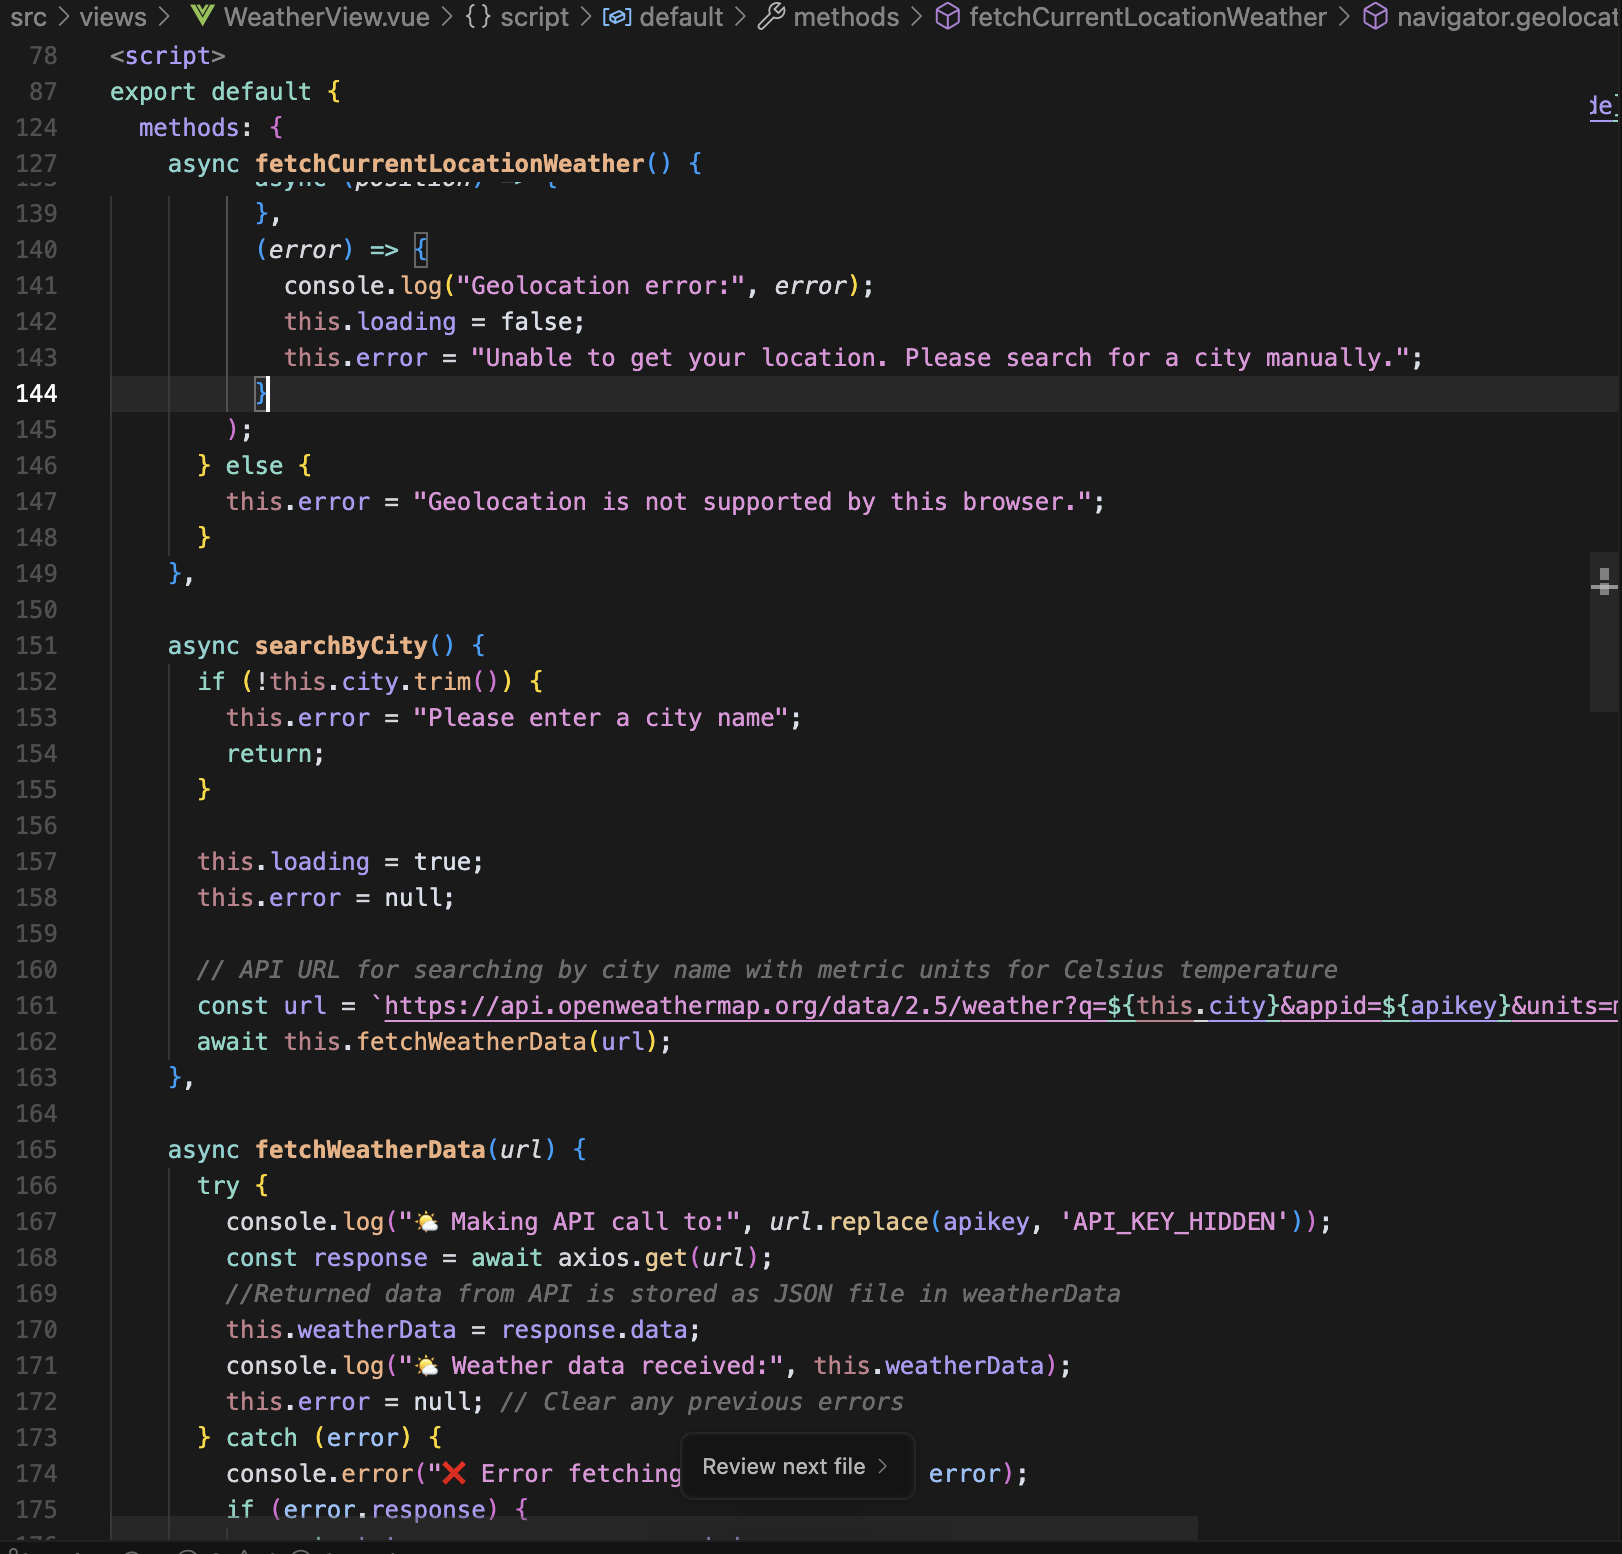
\includegraphics[width=0.9\textwidth]{weather_search_code.png}
\caption{WeatherView.vue - searchByCity function implementation with API call}
\end{figure}

\subsubsection{Browser Display - Clayton Weather Search}
% Screenshot showing Clayton, AU weather search results
% 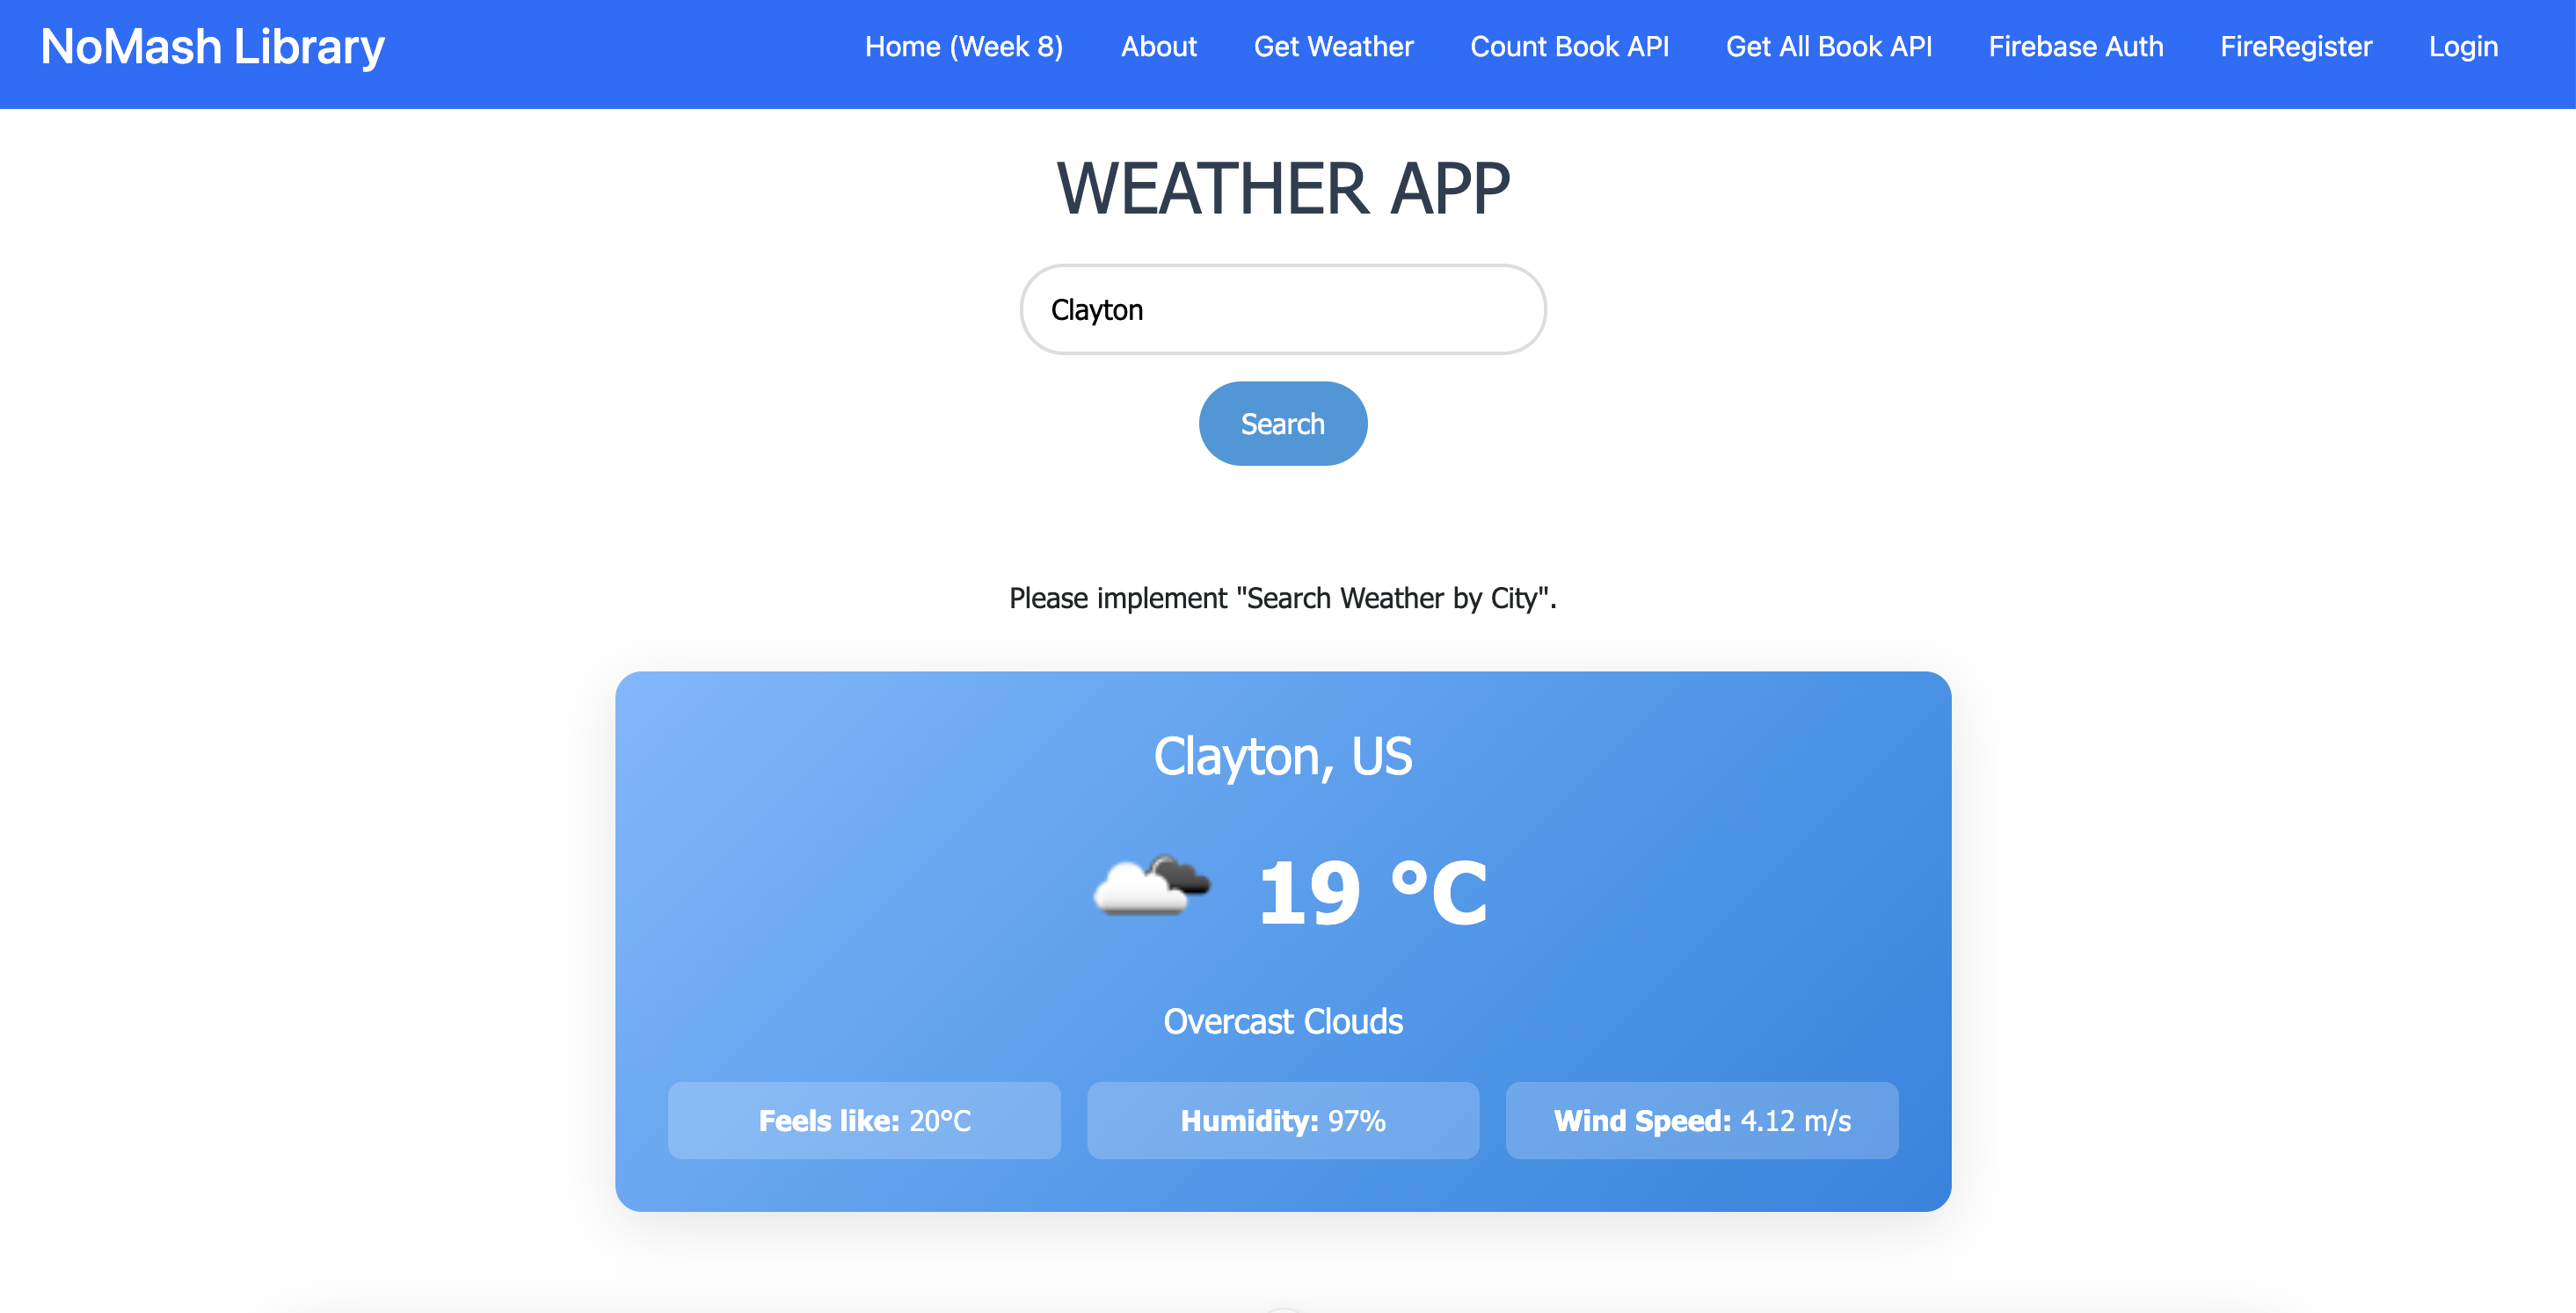
\includegraphics[width=0.9\textwidth]{clayton_weather_search.png}
\begin{figure}[H]
\centering
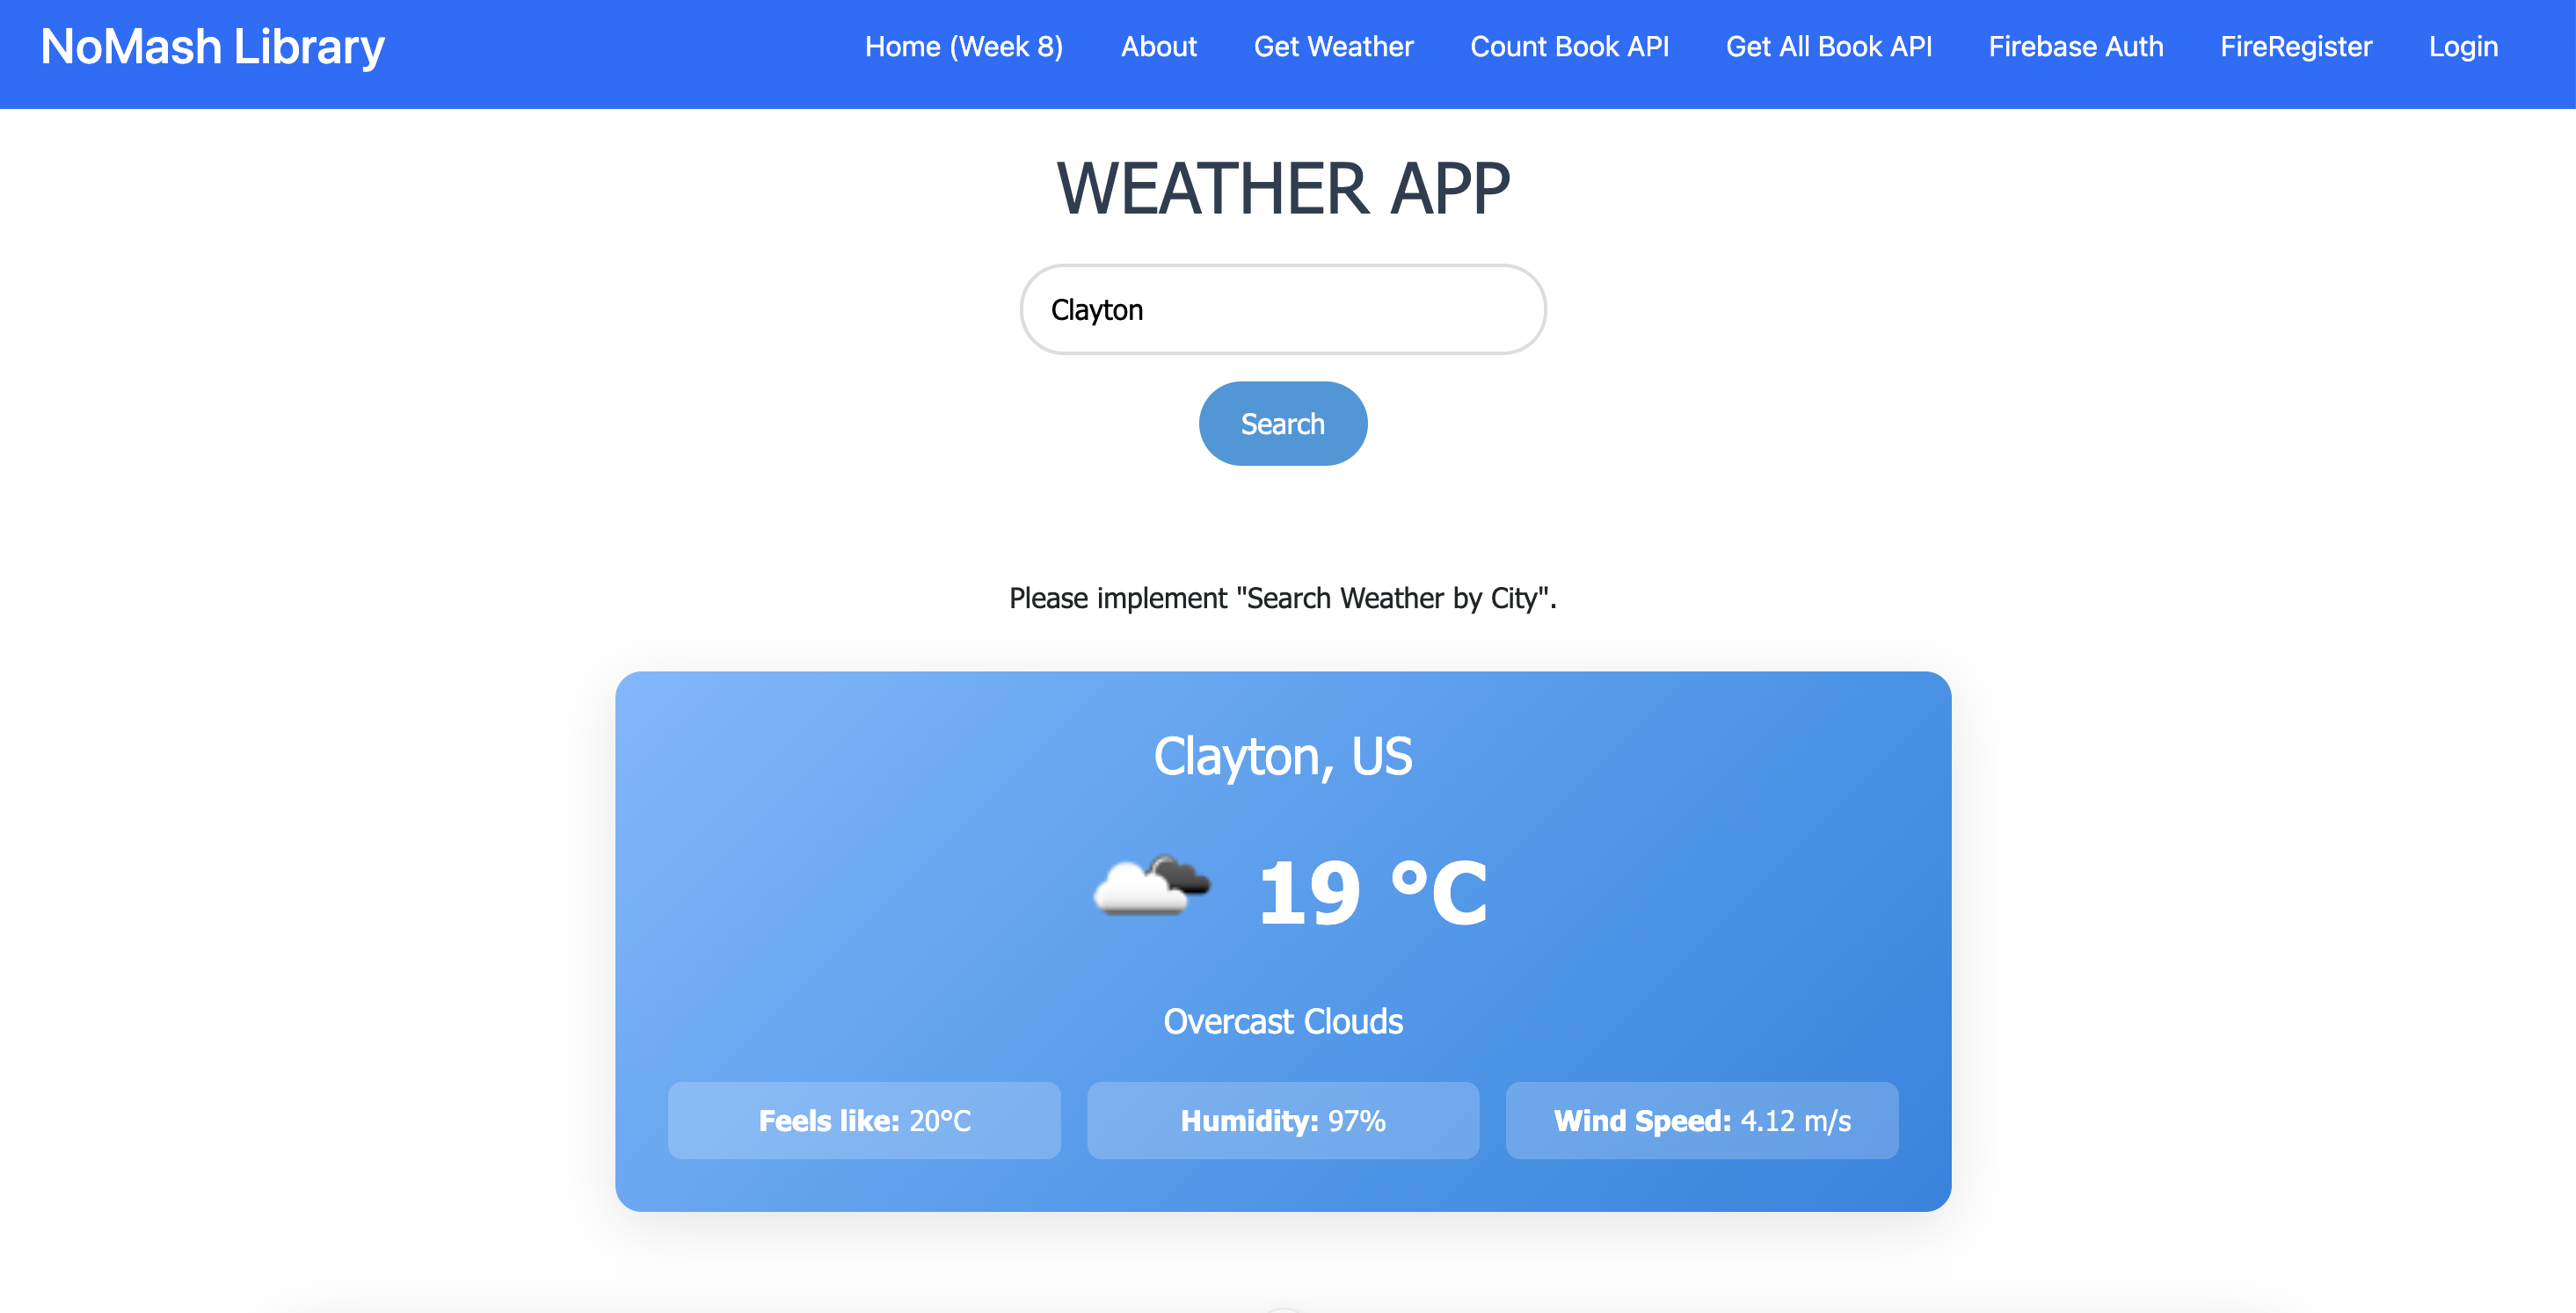
\includegraphics[width=0.9\textwidth]{clayton_weather_search.png}
\caption{Browser showing Clayton, AU weather search with temperature in Celsius and weather icon}
\end{figure}

\subsection{Screenshot Set 2: GetAllBookAPI Implementation}

\subsubsection{GetAllBookAPI Code Implementation}
% Screenshot showing GetAllBookAPI implementation
% 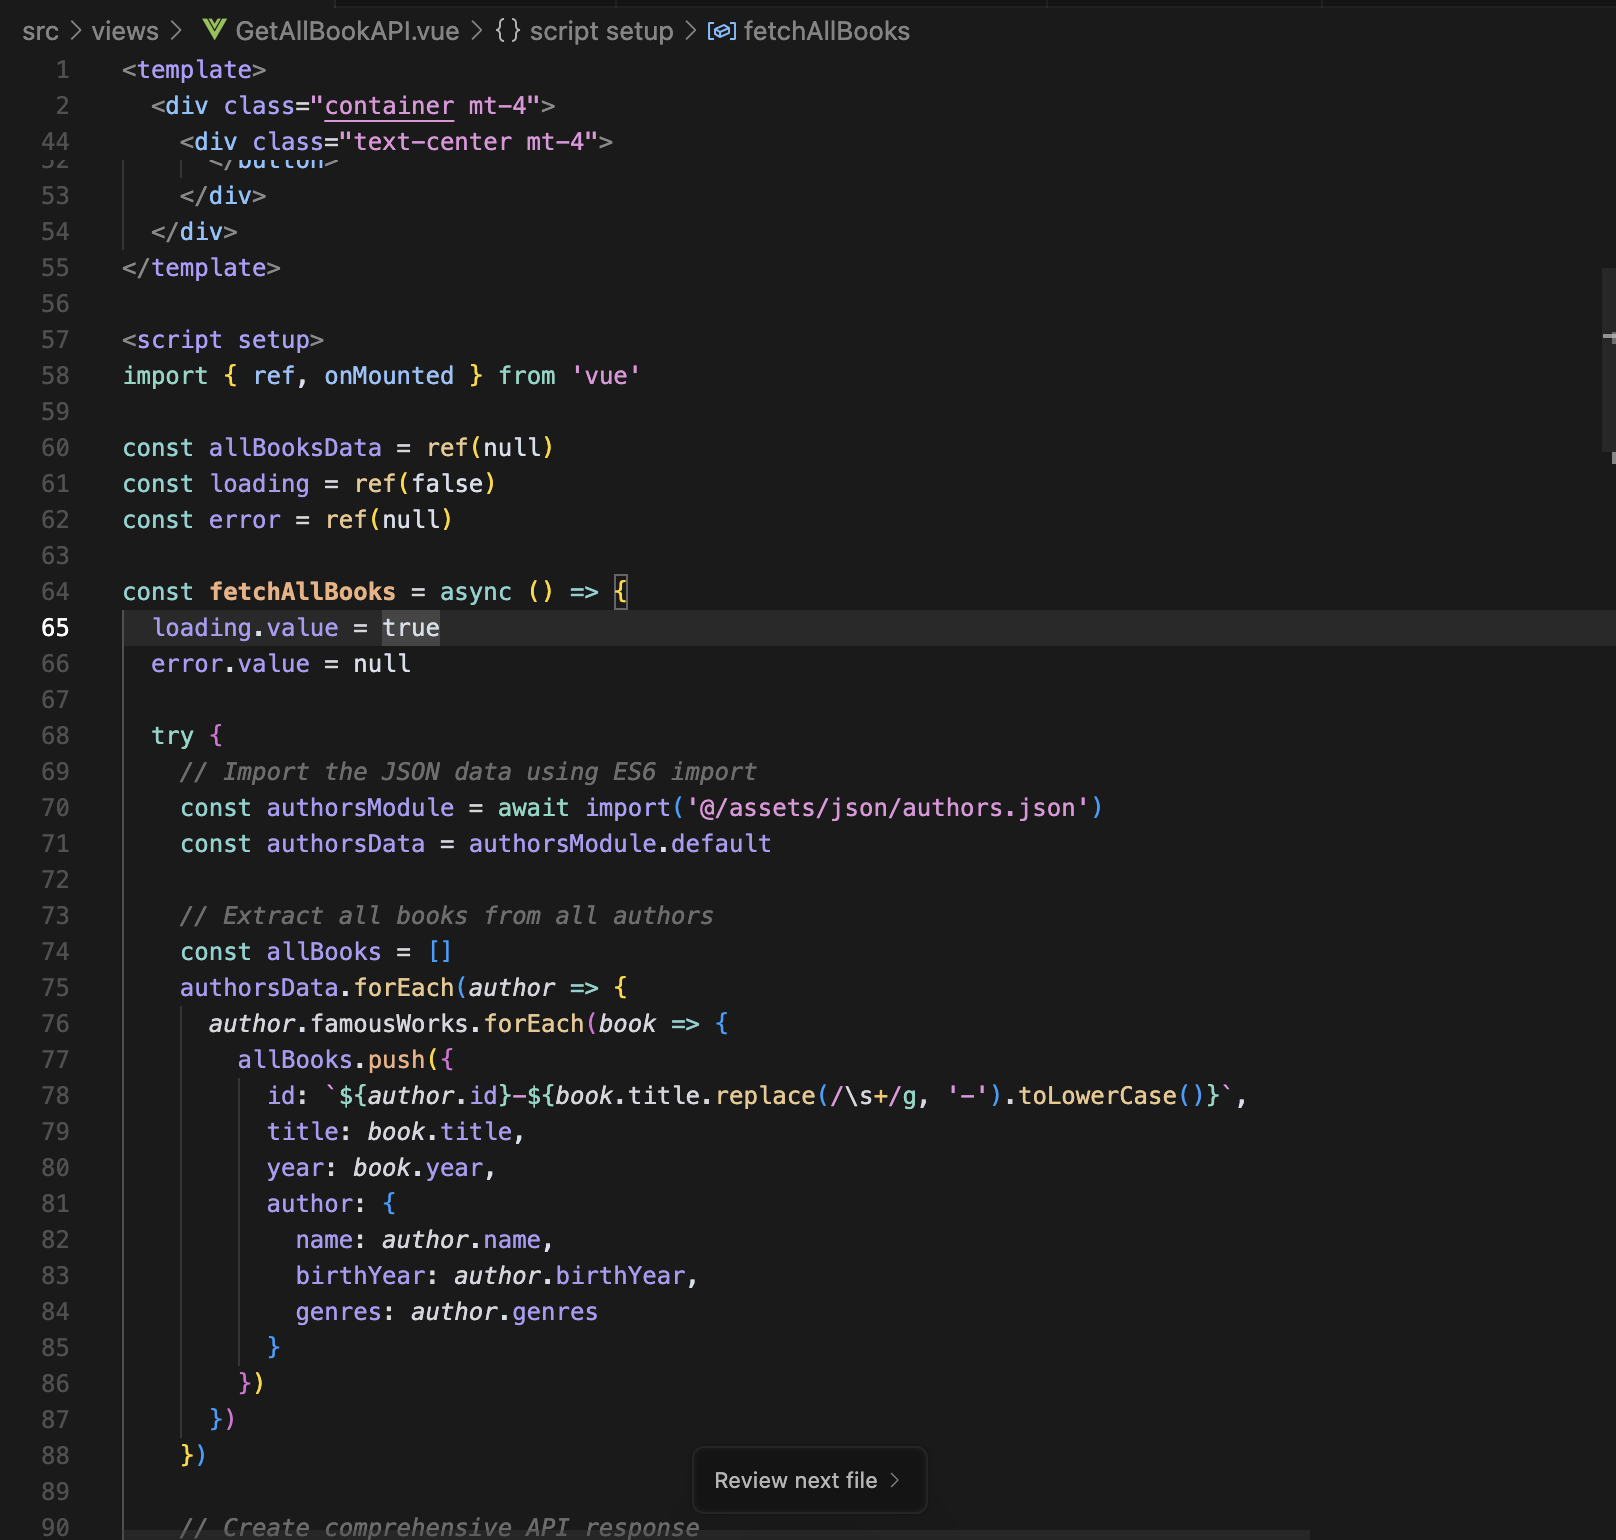
\includegraphics[width=0.9\textwidth]{getallbook_api_code.png}
\begin{figure}[H]
\centering
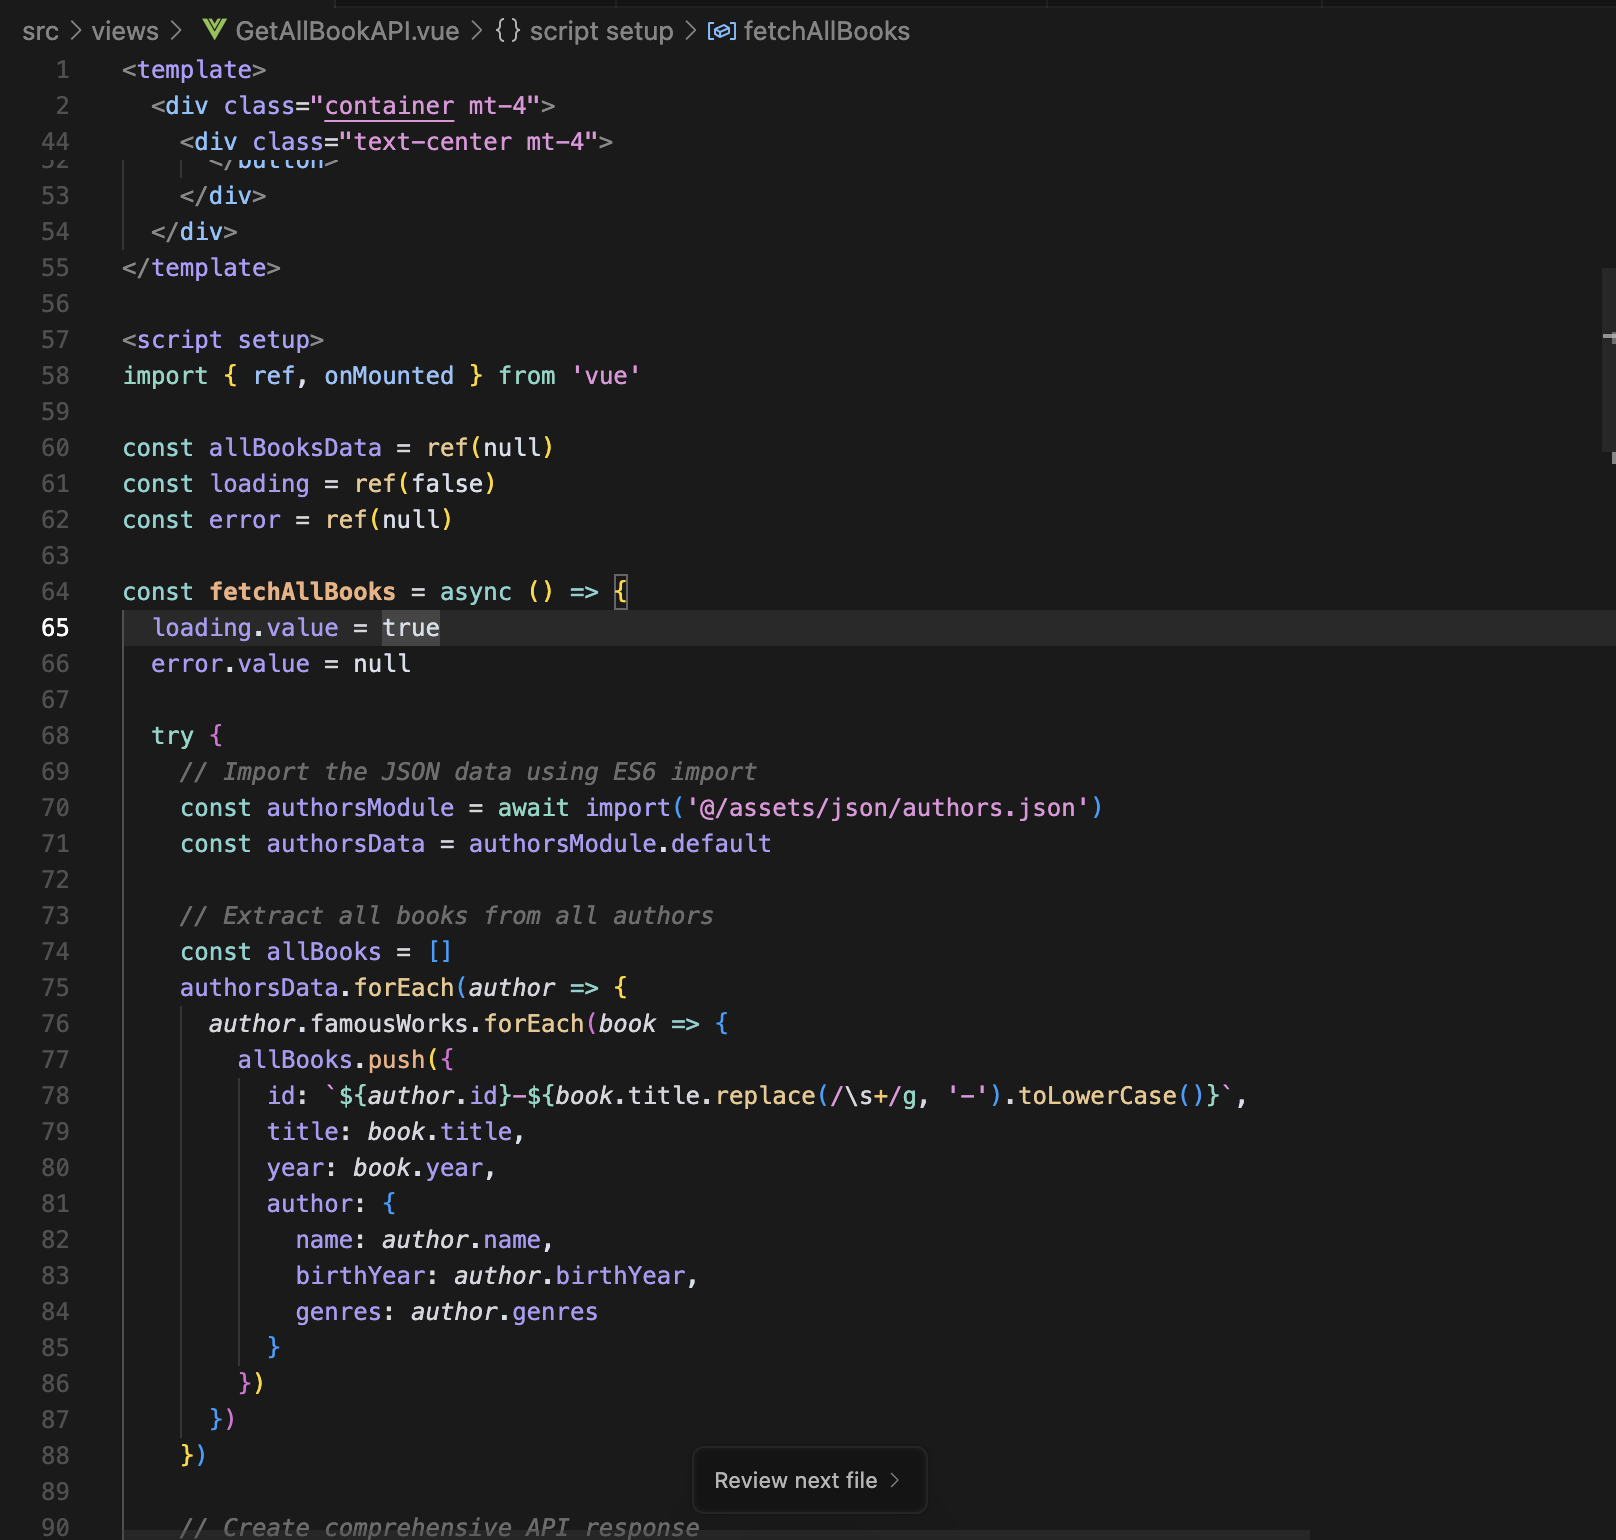
\includegraphics[width=0.9\textwidth]{getallbook_api_code.png}
\caption{Implementation code for GetAllBookAPI showing JSON data retrieval and formatting}
\end{figure}

\subsubsection{Browser Display - All Books JSON Format}
% Screenshot showing all books in JSON format
% 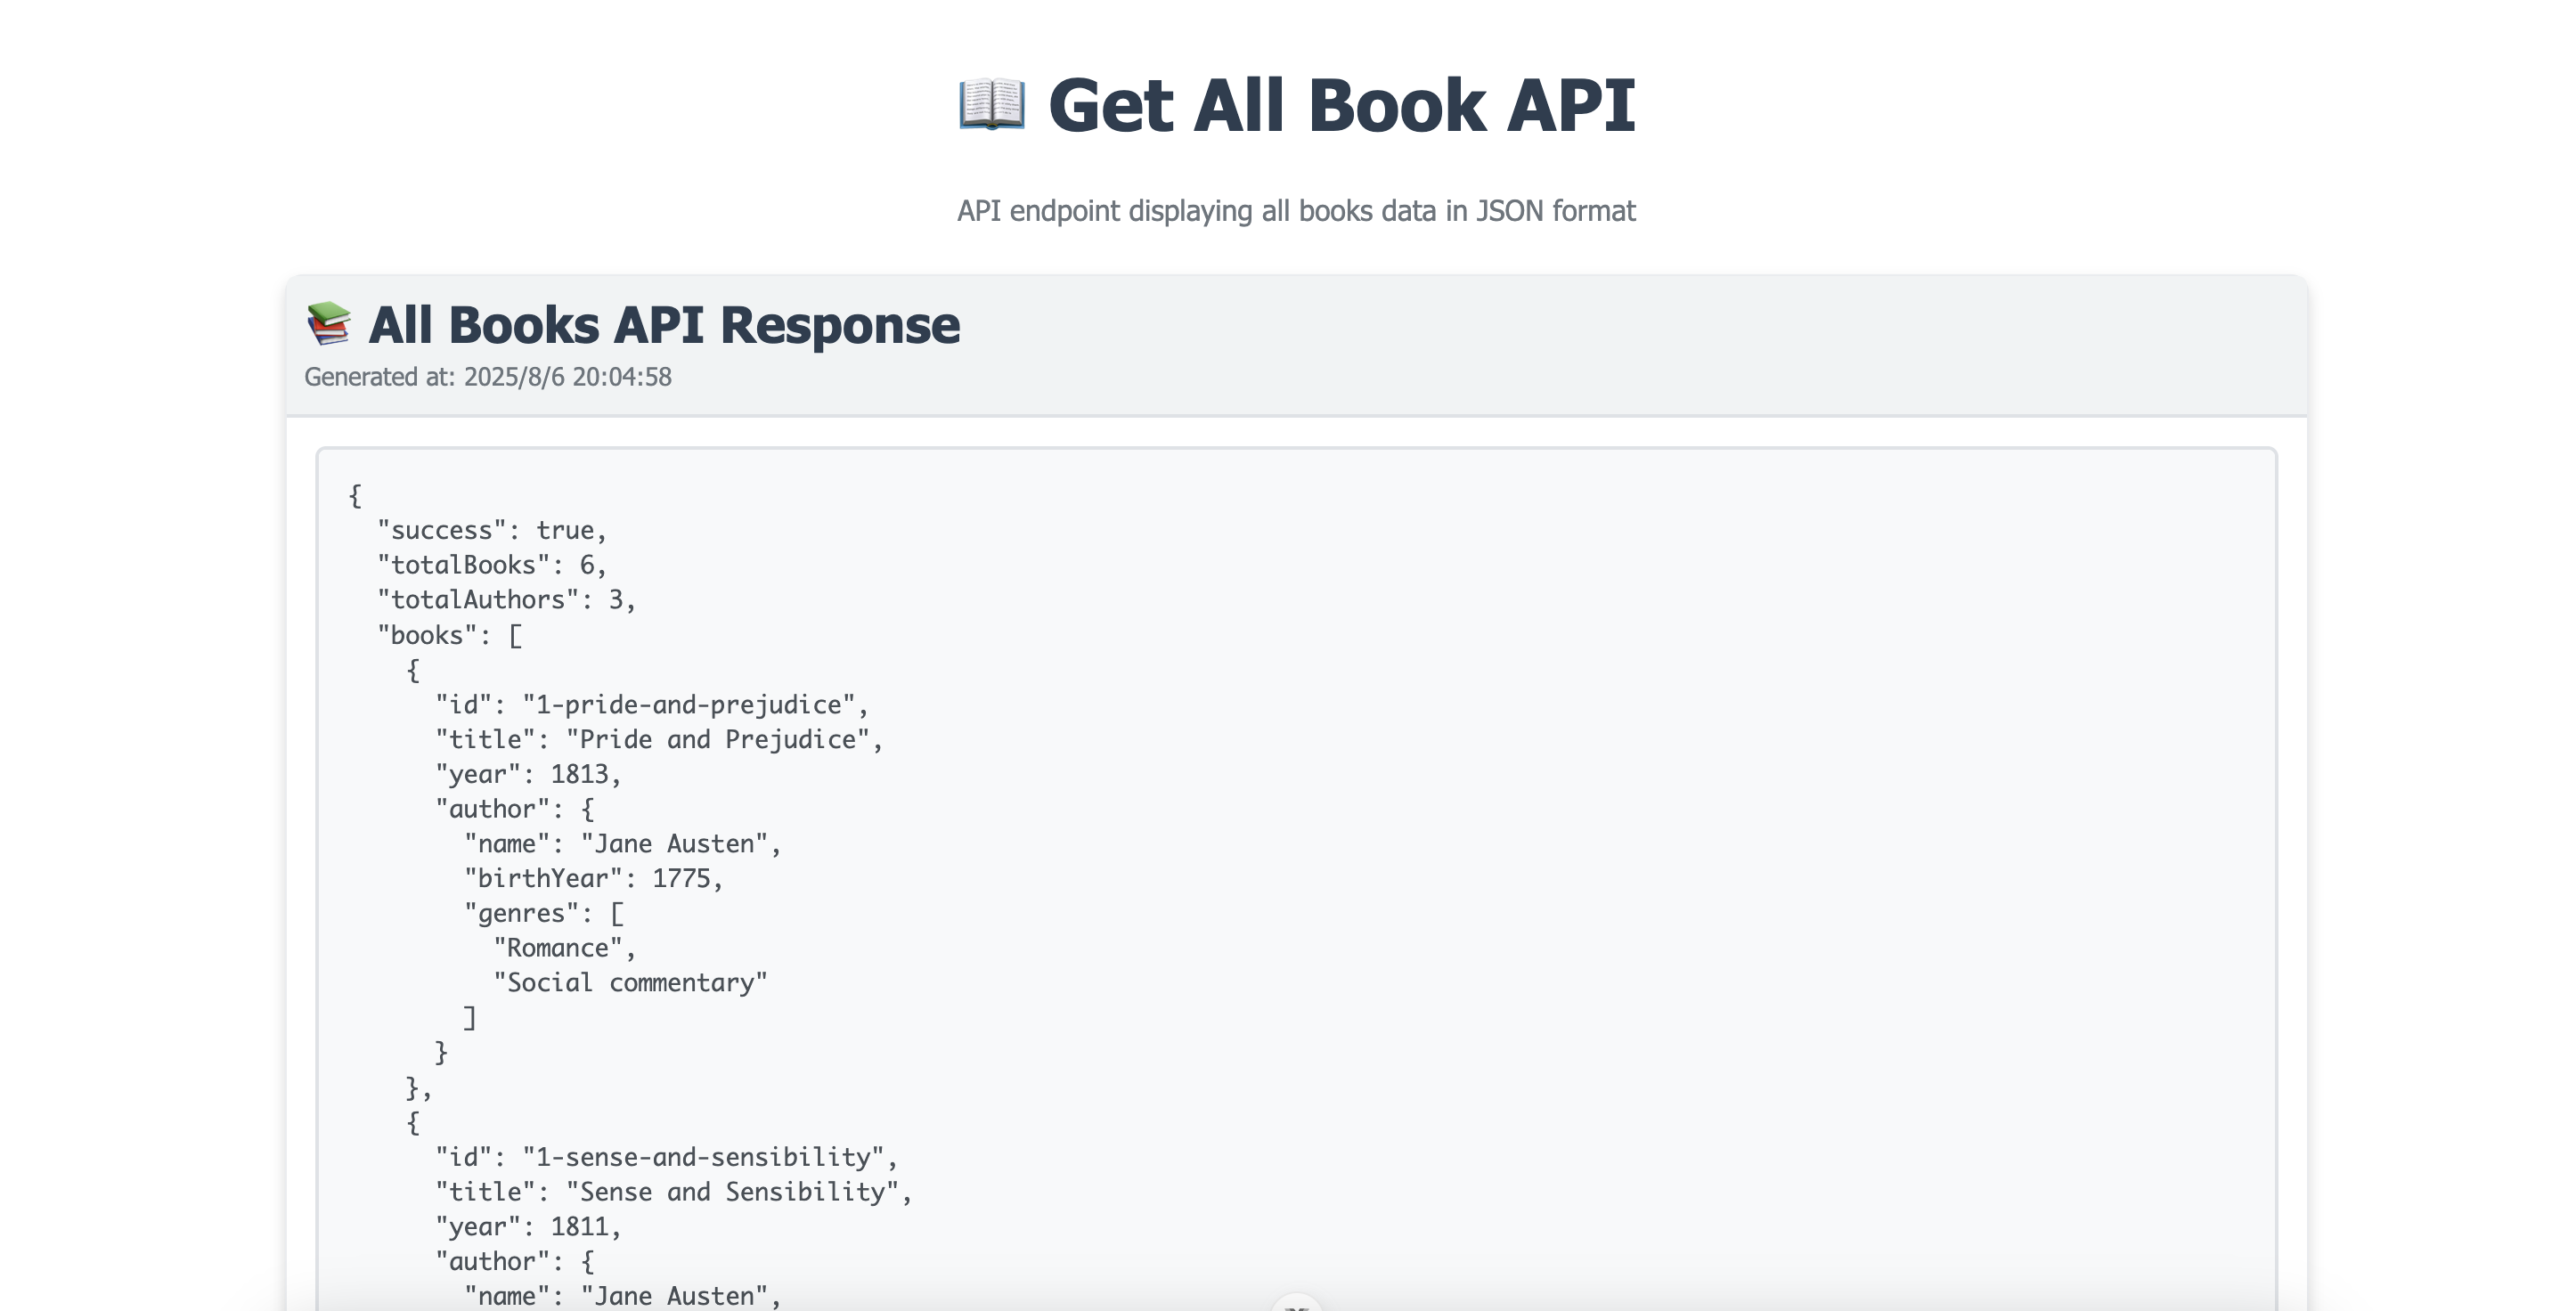
\includegraphics[width=0.9\textwidth]{all_books_json_browser.png}
\begin{figure}[H]
\centering
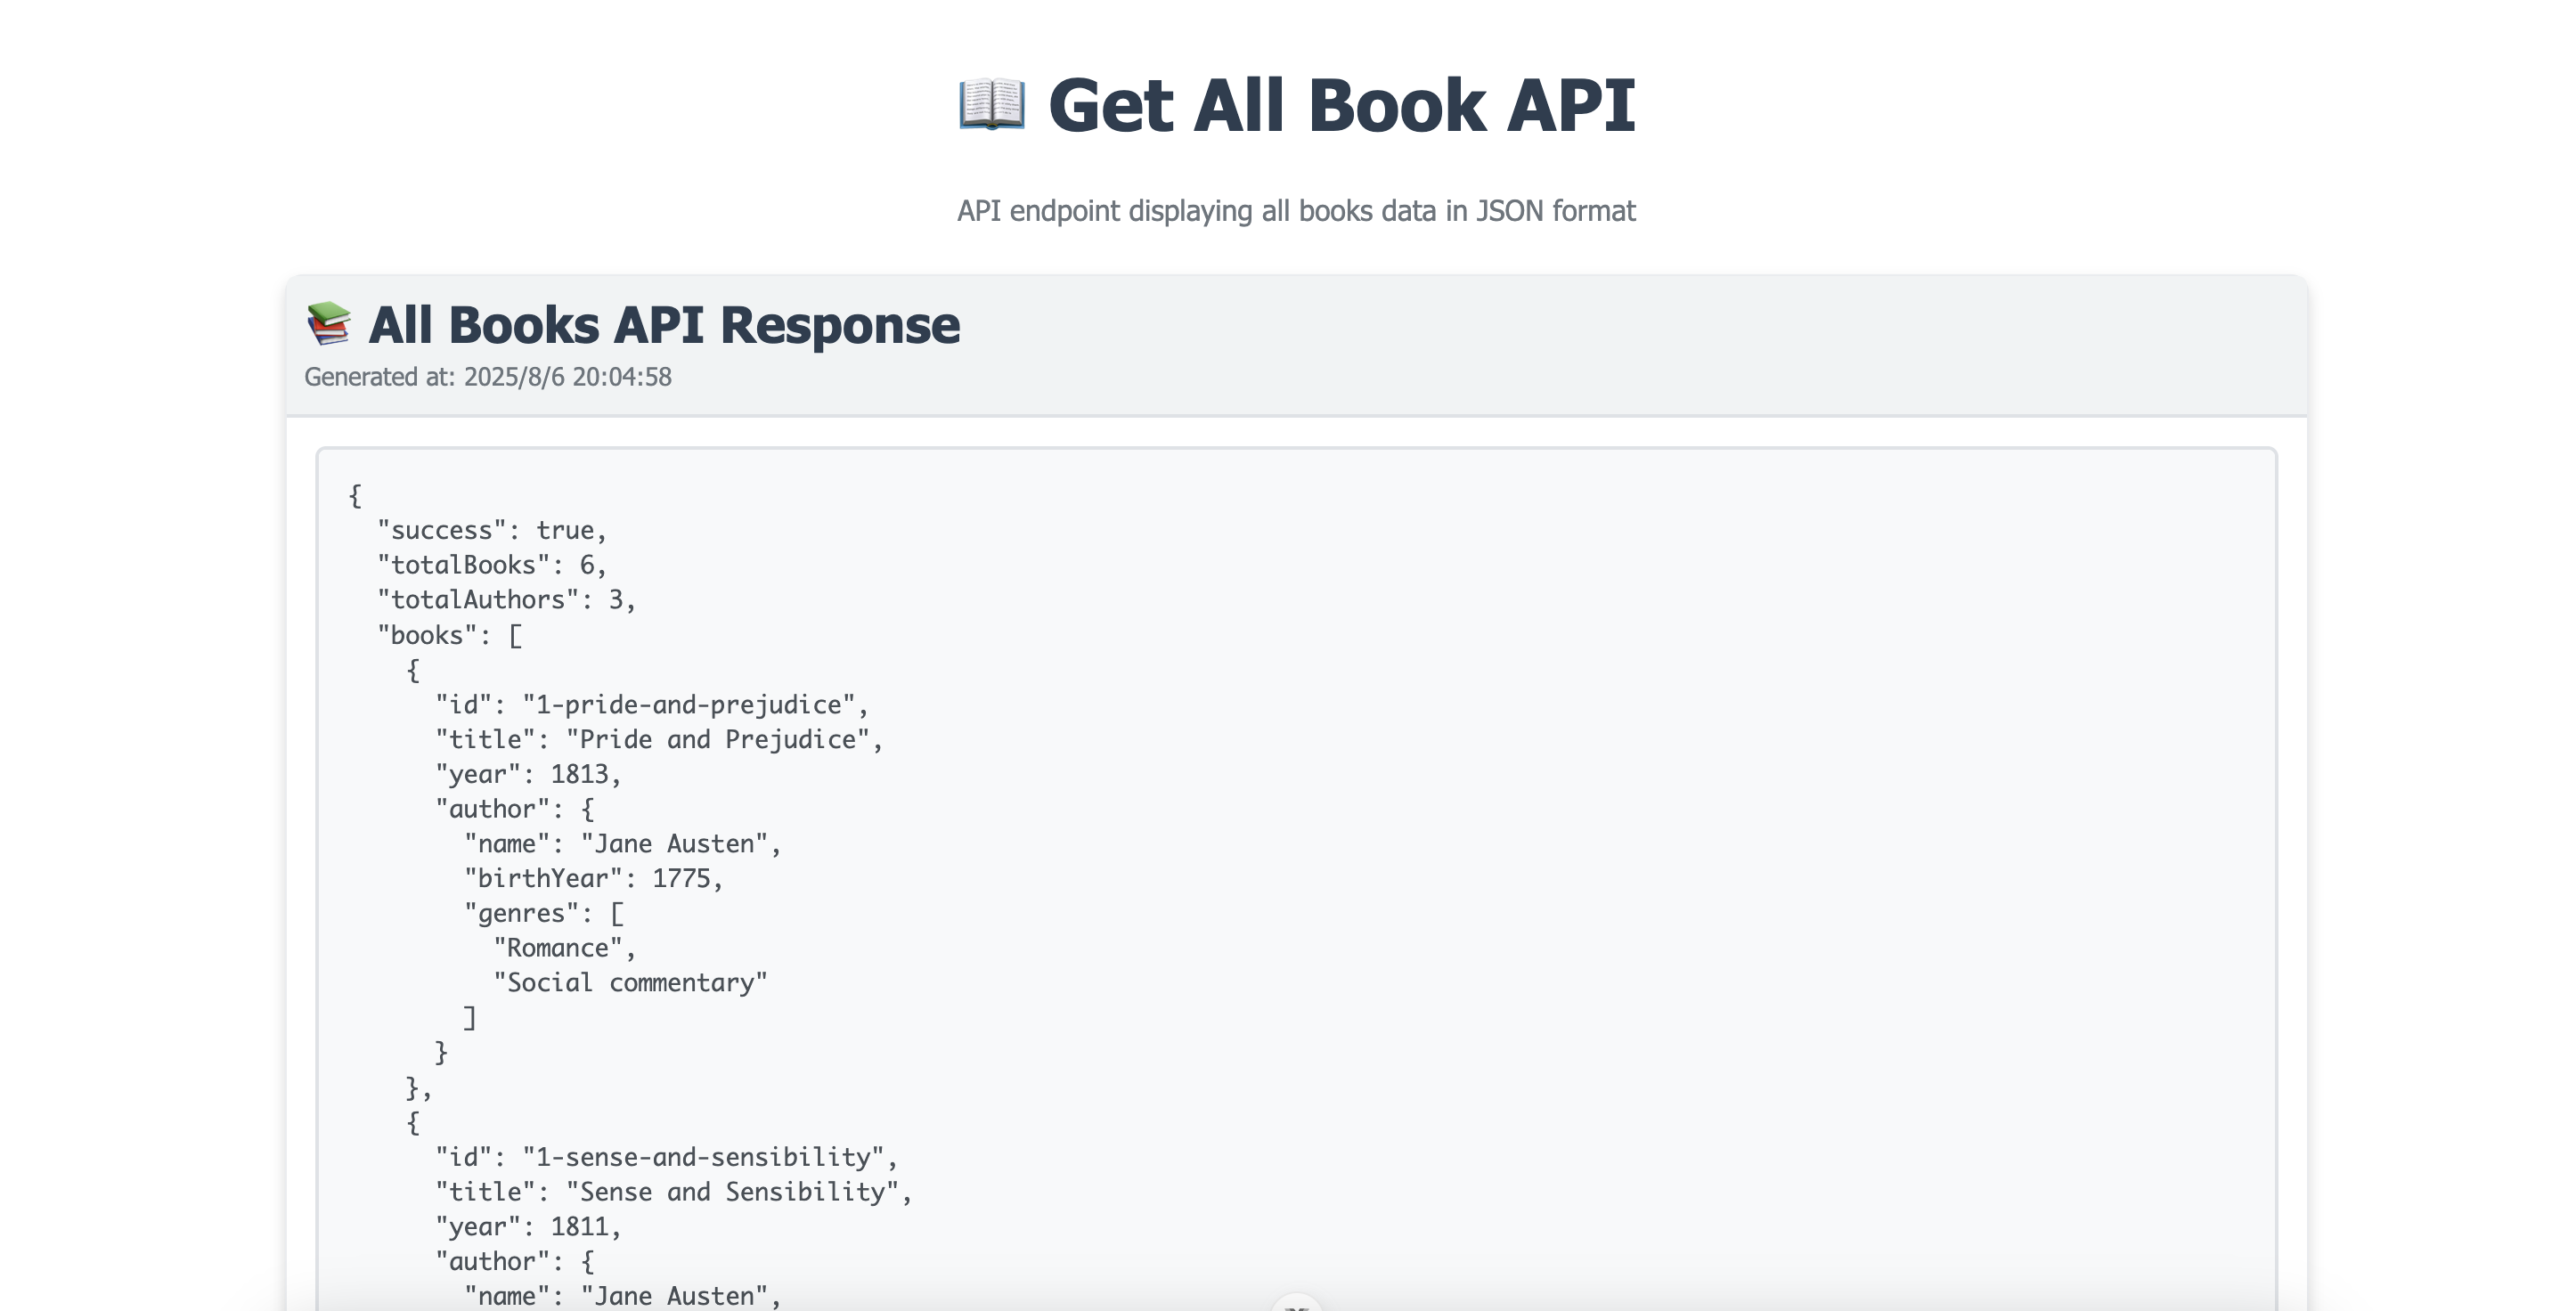
\includegraphics[width=0.9\textwidth]{all_books_json_browser.png}
\caption{Browser view showing all books data in JSON format on GetAllBookAPI page}
\end{figure}

\newpage



\section{Key Implementation Features}

\subsection{External API Integration}
\begin{itemize}
\item OpenWeatherMap API integration with personal API key
\item Geolocation-based current weather fetching
\item City-based weather search functionality
\item Temperature display in Celsius with weather icons
\item Error handling for API failures and invalid cities
\end{itemize}

\subsection{Local API Development}
\begin{itemize}
\item JSON data processing from authors.json file
\item Statistics calculation (authors count, total books)
\item API response formatting with metadata
\item Real-time data refresh functionality
\item Responsive UI with Bootstrap styling
\end{itemize}

\subsection{Technical Implementation}
\begin{itemize}
\item Vue 3 Composition API usage
\item Axios for HTTP requests
\item ES6 import for local JSON data
\item Router configuration for SPA navigation
\item Component-based architecture
\end{itemize}

\end{document} 